\documentclass[11pt]{article}

\usepackage[T1]{fontenc}
\usepackage[margin=1in]{geometry}
\usepackage{amsmath,amssymb,mathtools,amsthm}
\usepackage{booktabs,tabularx,array}
\usepackage{graphicx}
\usepackage{float}
\IfFileExists{lmodern.sty}
  {\usepackage{lmodern}\usepackage{microtype}}
  {\usepackage[expansion=false]{microtype}}
\usepackage{enumitem}
\usepackage[hidelinks]{hyperref}

\setlength{\parindent}{0pt}
\setlength{\parskip}{0.55em}
\setlist[itemize]{leftmargin=*,itemsep=0.15em,topsep=0.25em}
\renewcommand{\arraystretch}{1.12}

\newcommand{\AP}{\operatorname{AP}}
\newcommand{\CNAP}{\operatorname{CNAP}}
\newcommand{\Regime}{\mathcal{R}}
\newcommand{\Assess}{\mathcal{A}}
\newcommand{\CSet}{\mathcal{C}}
\newcommand{\PSet}{\Pi_\star}
\newcommand{\Boot}{\mathcal{B}}
\newcommand{\E}{\mathbb{E}}
\newcommand{\Prb}{\mathbb{P}}
\newcommand{\APta}{\widetilde{\AP}}
\newcommand{\CNAPta}{\widetilde{\CNAP}}
\newcommand{\Sanc}{S^{\mathrm{anc}}}
\newcommand{\Psianc}{\Psi^{\mathrm{anc}}}
\newcommand{\Thetaanc}{\Theta^{\mathrm{anc}}}

\newtheorem{definition}{Definition}
\newtheorem{proposition}{Proposition}
\theoremstyle{remark}
\newtheorem*{remark}{Remark}

\title{Supported Model Replacement Across Target Prevalences\\
\large An Observed-Anchored Hierarchy for Empirical and Computational Challenge}
\author{Marcus A. Thomas}
\date{Methodological proposal}

\begin{document}

\maketitle

\begin{abstract}
A decision to replace an incumbent prediction model often begins with an
observed performance difference. A stronger claim asks whether that advantage
survives the conditions, empirical evaluations, and computational
perturbations under which the claimant has agreed that it may fail. These
challenges have different scientific identities. A target condition is
evaluated within a full evaluation, a computational replication recombines
the evidence represented in one empirical evaluation, and an admitted
empirical evaluation supplies another observed test of the claim.

We develop an observed-anchored hierarchy that preserves those identities. A
paired effect first faces every declared target condition. Several empirical
effects then face an across-evaluation challenge, which acts as a necessary
empirical gate. Only a claim that passes that gate proceeds to a declared
within-evaluation computational challenge. Every nested challenge retains the
effect actually observed in each selected empirical evaluation as a mandatory
anchor. Computational replication can therefore preserve or reduce the support
credited to the observed evidence, but cannot erase an observed failure or
multiply the number of empirical tests.

The construction yields supported magnitude and literal survival of a declared
effect floor. An exact survival representation shows that both summarize the
same complete nested challenges. We develop the method for a paired,
tie-averaged, prior-standardized form of average precision across target
prevalences. A finite-evidence replacement rule requires both the observed
empirical gate and, when declared, the full anchored assessment to clear
prespecified thresholds. The rule does not estimate a probability of success
in unseen evaluations. It records what survived the attempted refutations
actually represented by the assessment.

Bank Marketing illustrates the anchored one-evaluation boundary. ProteinGym
supplies 91 observed assay evaluations whose comparisons fail at the empirical
gate, making further computational challenge unnecessary for their verdicts.
\end{abstract}


\section{Performance claims and levels of challenge}
\label{sec:introduction}

Prediction systems often rank cases so that a selected set can receive further
attention. A radiology service may send its highest-scored images for review;
a screening program may investigate its highest-scored records first. The
composition of that selected set matters because it is what the decision maker
receives.

Separation and selected-set purity part company when prevalence changes.
Suppose a threshold selects $80\%$ of positive cases and $5\%$ of negative
cases. In a balanced population of 10,000 cases it returns 4,000 positives and
250 negatives, for precision $0.94$. In a population with $1\%$ positives, the
same threshold returns 80 positives and 495 negatives, for precision $0.14$.
Its true-positive and false-positive rates have not moved. The supply of
negative cases has, and that is enough to change the meaning of the selected
set.

Average precision aggregates precision as a ranking is traversed. Ordinary
empirical AP therefore evaluates the ranking at the positive fraction in the
evaluation data. A performance claim intended for several deployment
populations should therefore name the target prevalences within its scope.
No single convenient prevalence establishes a claim throughout a range, and an
average over prevalences permits a favorable population to compensate for an
unfavorable one.

Call $D_m$ a \emph{full empirical evaluation} when it contains the outcomes and
scores needed to evaluate every declared target condition on one set of units.
A second opportunity for failure remains inside each full empirical
evaluation. A conclusion may depend on the realized combination of represented
units. A declared computational procedure can expose that dependence by recombining
those units. Call each resulting derived collection a \emph{computational
evaluation}. It is distinct from the empirical evaluation from which it is
derived, and it is \emph{full} when it contains the outcomes and scores needed
to evaluate every declared target condition. It supplies an additional
challenge confined to the failure mechanisms represented in the empirical
evaluation from which it is derived. The unqualified phrase \emph{full
evaluation} refers to either a full empirical evaluation or a full
computational evaluation.

A third opportunity for failure arises across distinct full empirical
evaluations. An effect retained in one admitted evaluation may fail in another
collection of units or context, so a claim intended to survive such tests should
declare the regime that admits them.

These three routes of attempted refutation have different scientific
identities:
\begin{enumerate}
\item a \emph{condition challenge} asks how much of the claimed performance
effect survives every declared condition within a full evaluation;
\item a \emph{computational challenge} asks how much of the claimed
performance effect survives declared recombinations within one empirical
evaluation; and
\item an \emph{empirical challenge} asks how much of the claimed performance
effect survives across the evaluations admitted by the evaluation regime.
\end{enumerate}
They share a noncompensation principle: each declared challenge is evaluated
as a whole, so a favorable component cannot erase an unfavorable component
within that challenge.

The motivating application is model replacement. Candidate $A$ and incumbent
$B$ are evaluated on the same units, and larger paired effects favor the named
orientation.

At first, this nesting seems to prescribe an inside-out calculation: challenge
the conditions, then the computational recombinations, and finally the
empirical evaluations. That order would, however, allow derived computational
results to enter before the observed empirical evidence has established that
there is anything to preserve. Computational recombination can deepen the
challenge applied to an empirical evaluation, but it cannot repair an observed
empirical failure. The construction therefore reverses the last two steps. It
first asks what observed effect survives across the empirical evaluations.
Only a claim that survives that empirical challenge is then exposed to the
additional within-evaluation computational challenge. This difference between
structural nesting and evidential order motivates the observed anchor developed
below.

\begin{figure}[H]
\centering
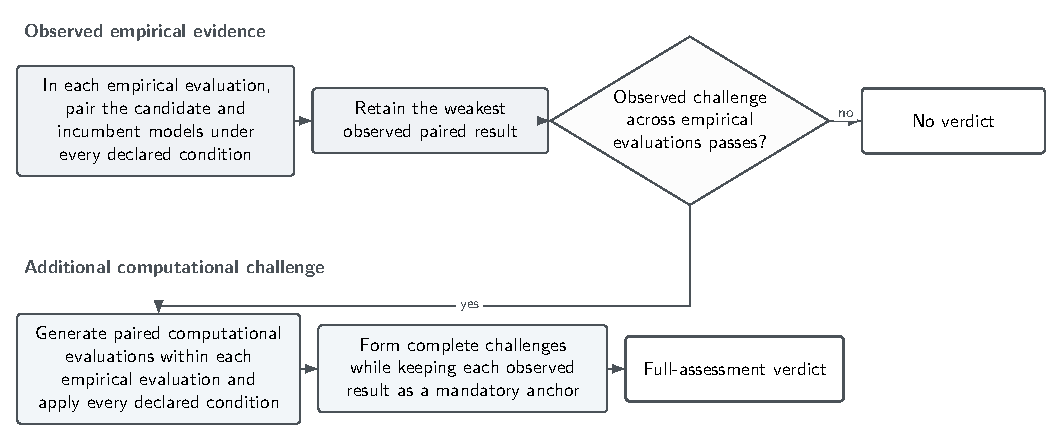
\includegraphics[width=\textwidth]{manuscript_images/observed-anchored-workflow.pdf}
\caption{Evidential order of the observed-anchored assessment. Each observed
or computational evaluation first faces every declared condition. The observed
empirical challenge is a necessary gate. Only a claim that passes that gate
proceeds to the additional within-evaluation computational challenge, with each
observed result retained as a mandatory anchor.}
\label{fig:assessment-workflow}
\end{figure}

In this construction, reproducibility is supported by specifying in advance
both what the effect is intended to survive and how demanding each challenge
will be. Five choices do this. The condition set $\CSet$ names the conditions
examined within every full evaluation. The empirical regime $\Regime$
determines which observed evaluations are admitted, their evaluation unit and
known dependence or multiplicity, whether their identities are retained rather
than pooled, and the rule by which they are selected. When a computational
challenge is included, $\Boot$ specifies how represented units are recombined
within each empirical evaluation. Finally, $K_E$ and $K_C$ specify the orders
of the empirical and computational challenges. We collect these choices in the
assessment specification
\[
\Assess
=
(\CSet,\Regime,\Boot,K_E,K_C).
\]
This specification declares the attempted refutations represented by the
assessment; it is not a stochastic model for how the observed data or unseen
evaluations were generated. Its elements belong to the claim and should be
fixed before the results are examined. If no scientifically defensible
computational procedure belongs to the assessment, the computational level is
absent; Section~\ref{sec:properties} gives the corresponding formal boundary.

The notation used below distinguishes the amount of empirical material or
computational approximation available from the severity of the challenge
applied to it. The counts $N_m$, $M$, and $J_m$ describe what is available; the
orders $K_E$ and $K_C$ describe how many effects are jointly faced:
\begin{center}
\begin{tabularx}{0.96\textwidth}{@{}l>{\raggedright\arraybackslash}X>{\raggedright\arraybackslash}X@{}}
\toprule
Symbol & Meaning & What increasing it changes \\
\midrule
$N_m$ & units in empirical evaluation $m$ & evidence represented within that evaluation \\
$M$ & admitted empirical evaluations & empirical tests and contexts available \\
$J_m$ & computational draws within evaluation $m$ & accuracy with which the declared within-evaluation challenge is approximated \\
$K_E$ & empirical challenge order & number of distinct empirical evaluations jointly faced \\
$K_C$ & computational challenge order & number of computational effects jointly faced within each selected evaluation \\
\bottomrule
\end{tabularx}
\end{center}
Thus, increasing $J_m$ refines the computational approximation, whereas
increasing $K_C$ changes the challenge itself. Likewise, increasing $M$ adds
empirical evidence, whereas increasing $K_E$ changes how the available
empirical evidence is challenged. No choice of $J_m$ turns one empirical
evaluation into several.

Pairing removes the possibility that the two models meet their adverse
conditions in different populations or evaluations. It also exposes a further
problem: finite-sample AP can reward whichever model divides tied scores more
finely, even when that refinement is unrelated to the outcomes.


\section{Constructing a retained paired AP effect}
\label{sec:paired-effect}

The hierarchy will act on effects that have already faced every declared target
condition.

\subsection{Prior-standardized average precision}

Let $D$ contain outcomes and the two fixed score vectors on a common set of
$N$ evaluation units. For a generic score $S$, write the observed
class-conditional selection rates at threshold $\tau$ as
\[
r(\tau)=\Prb_{\mathrm{obs}}(S\geq\tau\mid Y=1),
\qquad
f(\tau)=\Prb_{\mathrm{obs}}(S\geq\tau\mid Y=0).
\]
Prior standardization asks what precision these observed selection rates would
produce at a declared target prevalence
\[
\pi=\Prb_{\mathrm{target}}(Y=1)\in(0,1).
\]
The target population may therefore contain a different proportion of positive
cases than the observed evaluation. What is held fixed is the joint behavior
of the two model scores within each outcome class. Formally,
\begin{equation}
\Prb_{\mathrm{obs}}\{(S_A,S_B)\in G\mid Y=y\}
=
\Prb_{\mathrm{target}}\{(S_A,S_B)\in G\mid Y=y\},
\qquad y\in\{0,1\},
\label{eq:score-invariance}
\end{equation}
for every measurable $G\subseteq\mathbb R^2$. Here $G$ represents any
collection of possible paired scores. The equality says that among positive
cases ($Y=1$), the pair $(S_A,S_B)$ has the same distribution in the observed
and target populations, and likewise among negative cases ($Y=0$). Because the
equality holds for every $G$, it preserves both models' class-conditional score
distributions and their within-class association. Thus, the relative
prevalence of the two outcome classes may change, but the paired score behavior
within each class does not.

This score-level form of prior shift is weaker than invariance of $P(X\mid Y)$
but follows from it for fixed scoring rules
\cite{saerens2002adjusting,storkey2009training,lipton2018detecting}.

Under Equation~\eqref{eq:score-invariance}, Bayes' rule gives target precision
at threshold $\tau$:
\begin{equation}
p_\pi(\tau)
=
\frac{\pi r(\tau)}
{\pi r(\tau)+(1-\pi)f(\tau)}.
\label{eq:reference-precision}
\end{equation}
The evaluation supplies $r$ and $f$; the declared target population supplies
$\pi$. Aggregating this precision across the observed positive-class recall
increments gives prior-standardized AP, $\AP_\pi(D)$. Appendix~\ref{app:ap}
gives the empirical definition. Related calibration methods evaluate
precision-based metrics at a fixed reference class ratio
\cite{siblini2020calibration}. Here $\pi$ is instead a declared target-population
condition and may vary over $\PSet$.

Prior standardization does not transport changes within outcome class. If
severity, measurement, or features alter $P(S_A,S_B\mid Y)$, changing $\pi$
cannot represent the new context; the framework instead treats it as another
empirical evaluation admitted by $\Regime$
\cite{bareinboim2013transportability}.

\subsection{A common opportunity scale}

Population random ranking has $\AP_\pi=\pi$. Define
\begin{equation}
\CNAP_\pi(D)
=
\frac{\AP_\pi(D)-\pi}{1-\pi}.
\label{eq:cnap}
\end{equation}
CNAP is zero for population random ranking, one for perfect ranking, and
negative below chance. For two models,
\begin{equation}
\CNAP_{A,\pi}-\CNAP_{B,\pi}
=
\frac{\AP_{A,\pi}-\AP_{B,\pi}}{1-\pi}.
\label{eq:cnap-difference}
\end{equation}
A CNAP margin of a given size therefore requires a raw AP gain equal to that
size multiplied by $1-\pi$ at prevalence $\pi$. The scale is appropriate when
a replacement margin denotes a fraction
of the random-to-perfect opportunity rather than the same raw AP increment in
every target population \cite{cohen1960coefficient}.

This linear random-to-perfect normalization differs from
precision--recall-gain analysis, which uses harmonic gain coordinates and a
different integration measure \cite{flach2015prg}. CNAP retains the declared
target prevalence because selected-set purity in that population is the
quantity being challenged.

Common endpoints do not make the profile prevalence-invariant. At a threshold
with rates $r_h$ and $f_h$, the normalized contribution is
\begin{equation}
\frac{p_{\pi,h}-\pi}{1-\pi}
=
\frac{\pi(r_h-f_h)}
{\pi r_h+(1-\pi)f_h}.
\label{eq:threshold-cnap}
\end{equation}
Rare-positive populations charge false positives more heavily. Two models may
therefore exchange order as $\pi$ changes.

Let $\PSet\subset(0,1)$ be a nonempty compact target-prevalence set selected
from scientific knowledge or deployment plans before the paired profile is
examined. In the AP application, the condition index is $c=\pi$ and
$\CSet=\PSet$.

\subsection{Pair before challenging}

A replacement decision concerns an advantage under the same conditions. If
the two models are first summarized separately, the adverse prevalence may
differ between them and later subtraction will not recover the paired
advantage.

For one evaluation, let
\[
a=\inf_{\pi\in\PSet}\CNAP_{A,\pi},
\qquad
b=\inf_{\pi\in\PSet}\CNAP_{B,\pi},
\qquad
t=\inf_{\pi\in\PSet}
\{\CNAP_{A,\pi}-\CNAP_{B,\pi}\}.
\]
Then $a-b\geq t$. The separately challenged marginal reports can overstate the
advantage because they need not refer to the same prevalence. The same
noncomposition persists when effects are combined across evaluations;
Appendix~\ref{app:paired-proofs} gives the result.

The construction therefore pairs the models at each prevalence before taking
the condition infimum.

\subsection{Tie-averaged average precision}
\label{sec:tie-average}

Ordinary finite-sample AP also depends on how finely a score vector divides
ties. Stepwise AP is upward displaced under random ordering because it evaluates
precision when positive cases enter the ranking \cite{bestgen2015random}. A
fully tied outcome-blind score vector returns the random-ranking value, while
an outcome-blind vector of distinct scores creates more opportunities for
favorable positive entries. Pairing alone does not remove that advantage.

Let $\mathcal O(D)$ contain the strict rankings consistent with a score vector,
obtained by resolving each tied block in every possible order while preserving
the order between blocks.

\begin{definition}[Tie-averaged average precision]
\begin{equation}
\APta_\pi(D)
=
\frac{1}{|\mathcal O(D)|}
\sum_{o\in\mathcal O(D)}\AP_\pi(D_o),
\label{eq:tie-average}
\end{equation}
where $D_o$ is evaluation $D$ under strict ranking $o$. Define
$\CNAPta_\pi$ through Equation~\eqref{eq:cnap}.
\end{definition}

The convention represents outcome-blind random resolution within a score
block. It is appropriate when an operational cutoff may split the block and
the model supplies no further ordering information. Whole-block selection or
a prespecified informative secondary rule would define a different operational
regime.

Tie averaging remains responsive to informative refinement. A finer score
gains when it orders outcomes correctly within a coarse block and loses when it
orders them incorrectly. Only arbitrary refinement receives no expected
credit.

\begin{proposition}[Neutrality to arbitrary refinement]
\label{prop:refinement}
Suppose model $A$ preserves the order of model $B$'s score blocks and,
conditionally on $S_B$ and $Y$, its strict ranking is uniform over the rankings
consistent with $S_B$. Then, for every $\pi$,
\[
\E[\APta_{A,\pi}\mid S_B,Y]=\APta_{B,\pi}.
\]
\end{proposition}

The proposition conditions on the realized outcomes, so the coarse model may
itself be informative. Appendix~\ref{app:tie-computation} evaluates
Equation~\eqref{eq:tie-average} without enumerating tie resolutions.

\subsection{Observed and computational retained effects}

The paired effect profile in full evaluation $D$ is
\begin{equation}
\Delta^{A:B}_\pi(D)
=
\CNAPta_{A,\pi}(D)-\CNAPta_{B,\pi}(D).
\label{eq:paired-profile}
\end{equation}
Within empirical evaluation $D_m$, the observed retained effect is
\begin{equation}
z_m^{A:B,\mathrm{obs}}
=
\inf_{\pi\in\PSet}\Delta^{A:B}_\pi(D_m).
\label{eq:observed-retained}
\end{equation}
This is the largest paired advantage retained at every declared target
prevalence in the empirical evaluation. Its limiting prevalence may differ
between evaluations.

Let $D_m^{(j)}$ be computational replication $j$ generated from $D_m$ under
$\Boot$. Its retained effect is
\begin{equation}
z_{mj}^{A:B,\mathrm{comp}}
=
\inf_{\pi\in\PSet}\Delta^{A:B}_\pi(D_m^{(j)}).
\label{eq:computational-retained}
\end{equation}
To preserve pairing, the construction uses the same resampled units for both
models and throughout the prevalence profile. Resampling separately by model
destroys pairing; resampling separately by prevalence splices together
conditions from different computational evaluations.

The operations defining one entry are:
\[
\begin{aligned}
&\text{pair the models}
\longrightarrow
\text{apply outcome-blind tie handling}\\
&\qquad\longrightarrow
\text{challenge every target prevalence}
\longrightarrow
\text{retain the weakest paired effect}.
\end{aligned}
\]

\section{Support across empirical and computational challenges}
\label{sec:hierarchy}

The retained effects form a hierarchical array. Its rows are admitted
empirical evaluations. Each row has an observed retained effect and a list of
computational effects generated from that evaluation:
\begin{equation}
\begin{array}{c|c|cccc}
&\text{observed retained effect}&j=1&j=2&\cdots&j=J_m\\
\hline
D_1&z_1^{\mathrm{obs}}&z_{11}^{\mathrm{comp}}&z_{12}^{\mathrm{comp}}&\cdots&z_{1J_1}^{\mathrm{comp}}\\
D_2&z_2^{\mathrm{obs}}&z_{21}^{\mathrm{comp}}&z_{22}^{\mathrm{comp}}&\cdots&z_{2J_2}^{\mathrm{comp}}\\
\vdots&\vdots&\vdots&\vdots&\ddots&\vdots\\
D_M&z_M^{\mathrm{obs}}&z_{M1}^{\mathrm{comp}}&z_{M2}^{\mathrm{comp}}&\cdots&z_{MJ_M}^{\mathrm{comp}}
\end{array}
\label{eq:effect-array}
\end{equation}
Superscripts identifying $A:B$ are suppressed when the orientation is clear.
Every entry has already faced the complete condition challenge.

If a row's computational effects were allowed to replace its observed retained
effect, favorable recombinations could erase a failure that the empirical
evaluation actually exposed. Computation would then be called an additional
challenge even though it could make the assessment less adverse. To prevent
that reversal, the observed retained effect remains mandatory in every
challenge constructed from its row. In that role it is the row's
\emph{observed anchor}.

The remaining problem is to combine anchors and computational effects without
allowing computational multiplicity to masquerade as empirical replication.

\begin{figure}[htbp]
\centering
\fbox{\begin{minipage}{0.91\textwidth}
\centering
\textbf{One complete anchored challenge}\par
\vspace{0.35em}
select $K_E$ distinct empirical rows
$\longrightarrow$
retain each selected row's observed anchor\par
\vspace{0.35em}
$\longrightarrow$
select $K_C$ distinct computational effects within every selected row
$\longrightarrow$
take the minimum over the complete selected structure\par
\vspace{0.35em}
$\longrightarrow$
average only after all complete challenge minima have been formed
\end{minipage}}
\caption{The order of the hierarchical construction. Conditions have already
been challenged inside every displayed effect. Empirical rows and
computational cells retain their identities throughout the remaining steps.}
\label{fig:hierarchy-schematic}
\end{figure}

\subsection{The finite-list support operator}

\begin{definition}[Finite-list survival support]
\label{def:support}
For a finite list $\mathbf t=(t_1,\ldots,t_L)$ and $1\leq K\leq L$, let
\[
\mathcal I_{L,K}
=
\{I\subseteq\{1,\ldots,L\}:|I|=K\}.
\]
Define
\begin{equation}
S_K(\mathbf t)
=
\binom{L}{K}^{-1}
\sum_{I\in\mathcal I_{L,K}}
\min_{\ell\in I}t_\ell.
\label{eq:finite-list-support}
\end{equation}
The entries may be effects from admitted empirical evaluations, empirical
replications, or computational replications. Their scientific source and
evidential identity should be stated whenever the operator is used.
\end{definition}

The operator forms each complete distinct order-$K$ subset, records its weakest
effect, and only then averages. At $K=1$ it is the list mean. At $K=L$ it is
the observed minimum. Increasing $K$ moves influence toward the lower entries
without asserting a probability law for an unseen list.

For observed anchors
$\mathbf z^{\mathrm{obs}}=(z_1^{\mathrm{obs}},\ldots,z_M^{\mathrm{obs}})$,
\begin{equation}
\theta^{\mathrm{obs}}_{A:B;K_E}
=
S_{K_E}(\mathbf z^{A:B,\mathrm{obs}})
\label{eq:observed-support}
\end{equation}
is direct observed support across the admitted empirical evaluations.
It will serve as the empirical gate for the full hierarchy.

\subsection{One complete nested challenge}

For each selected empirical evaluation $m$, let
$A_m\subseteq\{1,\ldots,J_m\}$ contain the $K_C$ distinct computational
indices selected from that row, so $|A_m|=K_C$. The weakest effect contributed
by that row is
\[
\min\left\{
z_m^{\mathrm{obs}},
\min_{j\in A_m}z_{mj}^{\mathrm{comp}}
\right\}.
\]
Every such rowwise challenge includes the observed anchor. The computational
entries add opportunities to expose fragility, but they cannot remove the
empirical effect actually obtained.

Now choose $K_E$ distinct empirical evaluations, indexed by $I$. One complete
nested challenge returns
\[
\min_{m\in I}
\left\{
z_m^{\mathrm{obs}},
\min_{j\in A_m}z_{mj}^{\mathrm{comp}}
\right\}.
\]
Thus a challenge selects rows, selects computational effects within every
selected row, retains the observed anchors, and credits the claim only with the
weakest effect anywhere in that selected structure.

A small array makes the order visible:
\[
\begin{array}{c|c|ccc}
&z_m^{\mathrm{obs}}&z_{m1}^{\mathrm{comp}}&z_{m2}^{\mathrm{comp}}&z_{m3}^{\mathrm{comp}}\\
\hline
D_1&0.30&0.50&0.10&0.40\\
D_2&0.20&0.25&0.35&-0.05
\end{array}
\]
Take $K_E=2$ and $K_C=1$. Retaining the observed anchor from each row and
selecting the first computational effect from each row gives
\[
\min\{0.30,0.50,0.20,0.25\}=0.20.
\]
Selecting the second effect in $D_1$ and the third in $D_2$ gives
\[
\min\{0.30,0.10,0.20,-0.05\}=-0.05.
\]
There are nine complete computational selections. Averaging their anchored
minima gives $0.85/9=0.094\overline4$. By contrast, direct observed order-2
support uses only the two observed anchors:
\[
\min\{0.30,0.20\}=0.20.
\]
This happens to equal the minimum of the first displayed nested selection
because the $0.20$ observed anchor is the weakest entry in that selection. The
computational layer has deepened the challenge without creating more than the
two empirical tests represented by the rows.

\subsection{Observed-anchored nested support}

\begin{definition}[Observed-anchored nested support]
\label{def:anchored-support}
Allow empirical evaluation $m$ to contain $J_m$ computational effects. For
$1\leq K_E\leq M$ and
$1\leq K_C\leq\min_{1\leq m\leq M}J_m$, define
\begin{align}
&\Sanc_{K_E;K_C}
\left(\mathbf z^{\mathrm{obs}};\mathbf Z^{\mathrm{comp}}\right)
\notag\\
&\quad=
\binom{M}{K_E}^{-1}
\sum_{I\in\mathcal I_{M,K_E}}
\left\{
\prod_{m\in I}\binom{J_m}{K_C}
\right\}^{-1}
\notag\\
&\qquad\qquad\times
\sum_{\substack{
(A_m)_{m\in I}\\
A_m\in\mathcal I_{J_m,K_C}}}
\min_{m\in I}
\left\{
z_m^{\mathrm{obs}},
\min_{j\in A_m}z_{mj}^{\mathrm{comp}}
\right\}.
\label{eq:anchored-support}
\end{align}
\end{definition}

The semicolon separates the empirical order from the computational order. For
a fixed empirical subset $I$, row $m$ offers $\binom{J_m}{K_C}$ distinct
order-$K_C$ subsets. A complete computational selection chooses one such
subset in every row, so $I$ admits
\[
\prod_{m\in I}\binom{J_m}{K_C}
\]
complete computational selections. For each one, the minimum is taken over
the observed anchors and all selected computational effects. Definition
\ref{def:anchored-support} averages these complete-selection minima---not
separate row summaries---conditional on $I$ and then averages uniformly over
the empirical subsets. The conditional normalization prevents an empirical
subset from receiving greater weight merely because its rows contain more
computational draws.

When every row contains the same number $J$ of computational effects,
$J_m=J$, the conditional number of complete selections becomes
\[
\prod_{m\in I}\binom{J}{K_C}
=
\binom{J}{K_C}^{K_E},
\]
and Definition~\ref{def:anchored-support} reduces to
\begin{align*}
&\Sanc_{K_E;K_C}
\left(\mathbf z^{\mathrm{obs}};\mathbf Z^{\mathrm{comp}}\right)\\
&\quad=
\frac{1}{\binom{M}{K_E}\binom{J}{K_C}^{K_E}}
\sum_{I\in\mathcal I_{M,K_E}}
\quad
\sum_{\substack{
(A_m)_{m\in I}\\
A_m\in\mathcal I_{J,K_C}}}
\min_{m\in I}
\left\{
z_m^{\mathrm{obs}},
\min_{j\in A_m}z_{mj}^{\mathrm{comp}}
\right\}.
\end{align*}

For the oriented paired AP comparison, write
\begin{equation}
\Thetaanc_{A:B;K_E,K_C}
=
\Sanc_{K_E;K_C}
\left(
\mathbf z^{A:B,\mathrm{obs}};
\mathbf Z^{A:B,\mathrm{comp}}
\right).
\label{eq:anchored-paired-support}
\end{equation}
A positive value means that the average weakest paired advantage over complete
nested challenges is positive.

The outer factor $\binom{M}{K_E}^{-1}$ in Definition
\ref{def:anchored-support} assigns equal weight to every distinct order-$K_E$
empirical subset. Consequently, every admitted empirical evaluation has the
same marginal inclusion weight $K_E/M$, regardless of its number of units,
computational draws, or the multiplicity of its broader context in the
collection. This uniform empirical weighting is a declared policy choice
within $\Regime$, not a consequence of the finite-evidence interpretation. It
prevents larger evaluations from dominating by unit count, but it does not
correct contextual multiplicity. A nonuniform empirical weighting would define
an extension of the present operator and is not used here.

\subsection{Why the hierarchy cannot be flattened or summarized by rows}

Flattening Equation~\eqref{eq:effect-array} into $\sum_mJ_m$ computational
entries would allow additional Monte Carlo draws from one evaluation to count
as additional empirical tests. It would also let the result change merely
because one row was assigned a larger approximation count. The empirical
index therefore remains intact in the construction.

Nor can the full operator be recovered by first averaging each row:
\begin{equation}
\Sanc_{K_E;K_C}
\ne
S_{K_E}\!\left(
\Sanc_{K_C}(z_1^{\mathrm{obs}};\mathbf z_1),
\ldots,
\Sanc_{K_C}(z_M^{\mathrm{obs}};\mathbf z_M)
\right),
\label{eq:row-noncomposition}
\end{equation}
where
\[
\Sanc_{K_C}(u;\mathbf t)
=
\binom{J}{K_C}^{-1}
\sum_{A\in\mathcal I_{J,K_C}}
\min\{u,\min_{j\in A}t_j\}.
\]
The right side averages within rows before applying cross-row minima. The full
operator instead takes the minimum of every complete nested challenge before
averaging.

In the numerical array above, the row summaries are
$0.70/3=0.233\overline3$ and $0.35/3=0.116\overline6$. Applying order-2
support to those two scalars gives $0.116\overline6$, not the correct nested
value $0.094\overline4$. Averaging and cross-row minimization do not commute.

The same principle governed the paired effect: pair models, challenge
conditions, retain anchors, and construct the complete nested challenge before
any averaging occurs.

\subsection{Literal survival of a declared floor}

Supported magnitude retains the numerical minimum from every complete nested
challenge. A decision may also require that minimum to clear a declared floor
$d$.

At level $s$, let
\[
R_{m,s}
=
\sum_{j=1}^{J_m}
\mathbf 1\{z_{mj}^{\mathrm{comp}}>s\}.
\]
The fraction of computational order-$K_C$ subsets in row $m$ whose entries all
clear $s$ is
$\binom{R_{m,s}}{K_C}/\binom{J_m}{K_C}$. A row clears the level only if its
observed anchor also clears it. Define the row survival fraction
\begin{equation}
q^{\mathrm{anc}}_{m,K_C,s}
=
\mathbf 1\{z_m^{\mathrm{obs}}>s\}
\frac{\binom{R_{m,s}}{K_C}}
{\binom{J_m}{K_C}}.
\label{eq:row-survival}
\end{equation}
If the observed anchor fails, no favorable computational subset can rescue the
row.

When computational selections are independent across empirical rows, literal
survival of the complete nested challenge is
\begin{equation}
\Psianc_{K_E;K_C,s}
=
\binom{M}{K_E}^{-1}
\sum_{I\in\mathcal I_{M,K_E}}
\prod_{m\in I}q^{\mathrm{anc}}_{m,K_C,s}.
\label{eq:anchored-survival}
\end{equation}
At the decision floor $d$, this is the fraction of complete nested challenges
in which every selected observed anchor and every selected computational
effect exceeds $d$.

In the running example with $d=0$, the first row has survival one and the
second has survival $2/3$. Because both rows are selected at $K_E=2$, nested
literal survival is $2/3$. The negative computational effect is not averaged
against the favorable ones inside the challenges that contain it.

Let $e_k$ denote the elementary symmetric polynomial of degree $k$. Equation
\eqref{eq:anchored-survival} is equivalently
\begin{equation}
\Psianc_{K_E;K_C,s}
=
\frac{e_{K_E}\left(
q^{\mathrm{anc}}_{1,K_C,s},\ldots,
q^{\mathrm{anc}}_{M,K_C,s}
\right)}{\binom{M}{K_E}}.
\label{eq:elementary-symmetric}
\end{equation}
This form will also make exact finite-array computation possible without
enumerating every nested selection.

\subsection{Magnitude and survival describe the same challenges}

Because the effect array is finite, choose real numbers $a\leq b$ such that
every observed and computational effect lies in $[a,b]$. Every complete
challenge value $t$ then also lies in $[a,b]$, and
\[
t=a+\int_a^b\mathbf 1\{t>s\}\,ds.
\]
Average this identity over the same nested selections used in
Definition~\ref{def:anchored-support}.

\begin{proposition}[Nested magnitude--survival identity]
\label{prop:survival-identity}
\begin{equation}
\Sanc_{K_E;K_C}
\left(\mathbf z^{\mathrm{obs}};\mathbf Z^{\mathrm{comp}}\right)
=
a+
\int_a^b
\Psianc_{K_E;K_C,s}\,ds.
\label{eq:nested-survival-identity}
\end{equation}
\end{proposition}

Supported magnitude integrates the survival of complete nested challenges
across all effect levels. Literal survival evaluates the same curve at the
policy floor $d$. Anchoring one quantity but not the other would sever this
identity and make the two decision criteria refer to different challenges.

\subsection{Boundary cases and challenge properties}
\label{sec:properties}

Permit $K_C=0$ as the mathematical convention
\[
A_m=\varnothing,
\qquad
\min_{j\in\varnothing}z_{mj}^{\mathrm{comp}}=+\infty,
\qquad
\binom{J_m}{0}=1.
\]
Then
\begin{equation}
\Sanc_{K_E;0}
=S_{K_E}(\mathbf z^{\mathrm{obs}}),
\qquad
\Psianc_{K_E;0,d}
=\psi_{K_E,d}(\mathbf z^{\mathrm{obs}}),
\label{eq:observed-boundary}
\end{equation}
where
\[
\psi_{K_E,d}(\mathbf z^{\mathrm{obs}})
=
\frac{\binom{R_d^{\mathrm{obs}}}{K_E}}
{\binom{M}{K_E}},
\qquad
R_d^{\mathrm{obs}}
=
\sum_{m=1}^M\mathbf 1\{z_m^{\mathrm{obs}}>d\}.
\]
The phrase \emph{observed-only assessment} is preferable in prose;
$K_C=0$ is not a zero-order empirical replication.

When $M=1$, $K_E=1$ is forced and the full construction becomes
\begin{equation}
\Sanc_{1;K_C}
=
\binom{J_1}{K_C}^{-1}
\sum_{A\in\mathcal I_{J_1,K_C}}
\min\left\{z_1^{\mathrm{obs}},
\min_{j\in A}z_{1j}^{\mathrm{comp}}\right\}.
\label{eq:one-evaluation-boundary}
\end{equation}
Setting the anchor formally to $+\infty$ recovers the unanchored computational
projection. That projection remains a useful secondary
diagnostic, but it is not the primary finite-evidence rule developed here.

The principal cases are summarized below.
\begin{center}
\begin{tabularx}{0.96\textwidth}{@{}lX X@{}}
\toprule
Setting & Quantity & Role \\
\midrule
$M>1$, $K_C\geq1$ & $\Sanc_{K_E;K_C}$ & full empirical--computational assessment \\
$M=1$, $K_E=1$, $K_C\geq1$ & $\Sanc_{1;K_C}$ & anchored one-evaluation assessment \\
$K_C=0$ & $S_{K_E}(\mathbf z^{\mathrm{obs}})$ & empirical gate; reduced assessment if computation is omitted \\
anchor $=+\infty$ & unanchored construction & secondary computational projection \\
\bottomrule
\end{tabularx}
\end{center}

Every complete anchored challenge contains its observed anchors. Consequently,
the full construction cannot exceed the observed-only analysis.

\begin{proposition}[Anchored challenge domination]
\label{prop:anchor-domination}
For every admissible $K_E,K_C$ and floor $d$,
\begin{align}
\Sanc_{K_E;K_C}
\left(\mathbf z^{\mathrm{obs}};\mathbf Z^{\mathrm{comp}}\right)
&\leq
S_{K_E}(\mathbf z^{\mathrm{obs}}),
\label{eq:magnitude-domination}\\
\Psianc_{K_E;K_C,d}
&\leq
\psi_{K_E,d}(\mathbf z^{\mathrm{obs}}).
\label{eq:survival-domination}
\end{align}
The anchored quantities also do not exceed the otherwise identical unanchored
nested projection.
\end{proposition}

The condition set and both orders control different dimensions of severity.

\begin{proposition}[Hierarchical challenge monotonicity]
\label{prop:monotonicity}
Subject to the required list lengths, anchored support and literal survival at
a fixed floor cannot increase when $\CSet$ is enlarged, $K_C$ is increased, or
$K_E$ is increased.
\end{proposition}

The regime $\Regime$ has no such mechanical ordering. Changing it changes the
scientific scope of the empirical tests rather than merely strengthening a
fixed challenge.

\subsection{Orientation}

The reverse profile is
$\Delta^{B:A}_\pi(D)=-\Delta^{A:B}_\pi(D)$, but negation occurs before the
condition infima and all nested minima. The reverse anchored value is therefore
not generally the negative of the forward value.

\begin{proposition}[Nested orientation bound]
\label{prop:orientation}
When both orientations use the same evaluations, computational replications,
and nested selections,
\begin{equation}
\Thetaanc_{A:B;K_E,K_C}
+
\Thetaanc_{B:A;K_E,K_C}
\leq0.
\label{eq:orientation}
\end{equation}
\end{proposition}
The construction cannot support positive challenged advantages in both
directions. Both may be nonpositive because different conditions, empirical
evaluations, or computational effects defeat the two directional claims.

Reference behavior may be examined through a deliberately constructed
exchangeable-label randomization. Under full exchangeability and outcome-blind
tie handling, the expected condition-specific paired effect is zero and the
expected anchored supported value is nonpositive. This is a diagnostic
reference, not a presumed sampling law. Appendix~\ref{app:paired-proofs}
defines the randomization, gives the finite-list argument, and shows why
restricted label symmetries need not have the same anchor.

\section{A staged finite-evidence replacement rule}
\label{sec:decision}

The operator describes what survived the declared challenges. A fully
specified replacement policy also states how much retained advantage and how
much literal survival are sufficient.

Let $\delta\geq0$ be the smallest supported magnitude that would justify
replacement. Let $d\geq0$ be the floor used to define literal survival, and
let $\gamma\in(0,1)$ be the minimum acceptable survival fraction. These are
policy commitments, not confidence levels or quantities learned from the
effect array.

\subsection{Stage 1: the observed empirical gate}

The oriented claim passes the empirical gate only if
\begin{equation}
\theta^{\mathrm{obs}}_{A:B;K_E}>\delta
\qquad\text{and}\qquad
\psi^{\mathrm{obs}}_{A:B;K_E,d}>\gamma.
\label{eq:observed-gate}
\end{equation}
The magnitude requirement prevents a negligible but widespread advantage from
automatically justifying replacement. The survival requirement prevents large
favorable effects from compensating for too many observed failures at $d$.

Failure of either condition returns no verdict. It does not establish that the
incumbent is superior. By anchor domination, computation cannot reverse the
failure.

\subsection{Stage 2: the computational challenge}

If Stage 1 passes and $\Boot$ belongs to the declared assessment, the primary
full rule requires
\begin{equation}
\Thetaanc_{A:B;K_E,K_C}>\delta
\qquad\text{and}\qquad
\Psianc_{A:B;K_E,K_C,d}>\gamma.
\label{eq:full-rule}
\end{equation}
Passing the observed gate but failing Equation~\eqref{eq:full-rule} means that
the advantage obtained across the empirical tests did not survive the declared
computational recombinations of their represented units. Passing both stages
supports replacement under the full anchored assessment.

The sequence is an ordered set of attempted refutations:
\[
\begin{aligned}
&\text{paired condition challenge}
\longrightarrow
\text{observed empirical gate}\\
&\qquad\longrightarrow
\text{within-evaluation computational challenge}
\longrightarrow
\text{full-assessment verdict}.
\end{aligned}
\]
The observed gate is reported even when Stage 2 is primary because it shows
what the empirical evaluations establish directly and identifies where the
claim was defeated.

\subsection{Reduced assessment and reverse orientation}

If no scientifically defensible $\Boot$ is available, or if omission of the
computational level was prespecified for a practical reason, the analysis may
stop at Equation~\eqref{eq:observed-gate}. A passing verdict then applies to
the reduced observed-only assessment. It should not be described as passage of
the full anchored rule.

Computational infeasibility identified in advance can justify declaring a
reduced observed-only assessment. If Stage 2 belongs to the declared
assessment and causes the full rule to return no verdict, the analysis should
not subsequently omit Stage 2 and report the passing Stage 1 result as support
under a reduced assessment. Nor should a smaller positive $J_m$ be described
as a substantively weaker challenge; it is a noisier approximation to the same
declared target.

The reverse comparison is constructed from
$\Delta^{B:A}_\pi=-\Delta^{A:B}_\pi$ before all condition infima, anchors,
and nested minima. It faces the same staged rule, with orientation-specific
thresholds if the consequences are asymmetric. If neither direction passes,
the result is no verdict.

The rule applies to the finite evidence and attempted refutations identified
in $\Assess$. It does not estimate a probability that an unseen
evaluation will pass, and it does not convert a computational law into a law of
nature. Using the verdict for deployment requires an external premise that the
declared conditions, regime, resampling procedure, and transport commitments
are adequate for the contemplated use. The calculation exposes those
commitments; it does not certify them.

\section{Evidence and computational implementation}
\label{sec:evidence}

The hierarchy preserves a difference that no algebra should erase. Empirical
evaluations supply evidence. Computational replications act on that evidence
under a declared procedure. The same numerical effect may appear at either
level, but its index records a different attempted refutation.

\subsection{The empirical evaluation regime}

The regime $\Regime$ states when a full empirical evaluation is admitted as a
test of the claim. It includes the object under test, eligible populations,
measurement standards, available outcomes and scores, the empirical
evaluation unit, known dependence or multiplicity among evaluations, and the
pooling or selection rule.

An \emph{admitted empirical evaluation} is a full observed evaluation
satisfying $\Regime$. Admission means that the evaluation enters the declared
finite evidence under the stated selection rule; it does not by itself assert
statistical independence from the other admitted evaluations.

An admitted empirical evaluation is an \emph{empirical replication} only when
it was separately conducted, its units are disjoint from those of every other
replication, and its model construction and data collection followed a protocol
fixed independently of the other evaluations in the set. Resampling draws,
administrative partitions, cross-validation folds, and repeated analyses of the
same units remain analyses of the same empirical evaluation.

A fixed-model regime holds the fitted models and measurement process fixed
while admitting new evaluation units. A broader regime may admit distinct
environments or a prespecified model-updating procedure. When an earlier
evaluation prompts a later update, the evaluations form an adaptive sequence;
they are not a set of separate replications under the definition above.

Several admitted evaluations may occur in different contexts while addressing
the same scoped claim. Their identities should be retained when contextual
variation is scientifically meaningful. If dataset membership is merely
administrative and all units address one aggregate population, pooling may be
more appropriate. The regime supplies admissibility; it does not assert that
admitted evaluations are empirical replications or draws from a common
population law.

\subsection{The within-evaluation computational procedure}

The procedure $\Boot$ declares how computational evaluations are generated
within each empirical row. For the AP illustration, $\Boot$ samples with
replacement separately from the positive and negative units represented in
each empirical evaluation, drawing the declared number of units from each
class. It keeps both model scores attached to every sampled unit and evaluates
the complete paired prevalence profile. The class counts are therefore fixed
across computational evaluations. Bank Marketing uses the observed class
counts; a prospective projection may use planned counts. A design-preserving
resampling procedure for clustered or matched studies operates on declared
design blocks rather than their component observations.

The resampling law is a constructed computational measure on recombinations of
represented units. It can expose dependence on the realized mix of those
units. It cannot produce an unseen case type or a failure caused by a new
environment, measurement process, development run, or scoring mechanism.

If empirical evaluations have nonoverlapping units and are resampled
separately, independent computational selections across rows give the product
in Equation~\eqref{eq:anchored-survival}. If evaluations share units or
scientific considerations call for coordinating a perturbation across
contexts, the joint computational law should preserve the resulting
dependence. The direct challenge definition remains valid, but the product
representation may not.

\subsection{The empirical gate is an exact stopping rule}

Calculate the observed anchors and their direct order-$K_E$ summaries before
generating computational replications for the primary verdict:
\[
\theta^{\mathrm{obs}}_{A:B;K_E}
=S_{K_E}(\mathbf z^{A:B,\mathrm{obs}}),
\qquad
\psi^{\mathrm{obs}}_{A:B;K_E,d}
=\psi_{K_E,d}(\mathbf z^{A:B,\mathrm{obs}}).
\]
If either observed quantity fails its policy threshold, Proposition
\ref{prop:anchor-domination} proves that the full anchored rule also fails.
The primary analysis can stop with no verdict. This is not an approximation or
a computational convenience imposed after the result; it is a consequence of
keeping the empirical effects binding.

If the empirical gate passes, generate the computational effects within each
row and evaluate the full anchored quantities. Computational replications may
still be generated after a gate failure as secondary fragility diagnostics,
but they are unnecessary for the replacement verdict.

\subsection{Computational target and Monte Carlo approximation}

The finite array approximates a functional under the declared resampling law.
If one computational retained effect in row $m$ exceeds $s$ with probability
$p_m(s)$ under that law, then the idealized iid order-$K_C$ row survival is
\begin{equation}
q^{\mathrm{anc},\infty}_{m,K_C,s}
=
\mathbf 1\{z_m^{\mathrm{obs}}>s\}p_m(s)^{K_C}.
\label{eq:ideal-row-survival}
\end{equation}
The finite distinct-subset fraction
\[
\binom{R_{m,s}}{K_C}/\binom{J_m}{K_C}
\]
is a U-statistic approximation to that row target. This distinction explains
why $K_C$ is substantive while $J_m$ is numerical. Lowering $K_C$ weakens the
declared challenge; lowering $J_m$ makes the same target less accurately
approximated.

Monte Carlo error concerns only the approximation of the declared
computational construction. It is not sampling uncertainty about a latent
population effect. Accuracy can be assessed through repeated independent seeds
and increasing $J_m$; the resulting stability checks do not alter the
scientific meaning of the challenge.

When the condition challenge is defined over a continuous set, its infimum
also requires numerical approximation. Missing an interior minimum can raise a
computed retained effect, so numerical accuracy of the effect values should be
checked separately from Monte Carlo stability. Appendix~\ref{app:computation}
gives the exact finite-array algorithm and the corresponding numerical checks.

\section{Empirical illustrations}
\label{sec:illustrations}

Two illustrations occupy different positions in the hierarchy. Bank
Marketing begins with one temporal empirical evaluation. Its positive-control
comparison passes the observed gate and proceeds to the anchored computational
challenge; its close model comparison fails at the gate. ProteinGym supplies
91 observed assay evaluations, but all examined orientations fail the observed
gate. The second stage is therefore unnecessary for their verdicts.

Bank Marketing uses $\PSet=[0.01,0.50]$; ProteinGym uses
$\PSet=[0.01,0.90]$. Both use $\delta=d=0$ and $\gamma=0.81$. Bank
Marketing uses $K_E=1$ and, when Stage 2 is reached, $K_C=2$. ProteinGym
uses observed order $K_E=2$. These choices define the illustrated policies
and are not proposed as defaults.

\subsection{One empirical evaluation: Bank Marketing}
\label{sec:bank-illustration}

The UCI Bank Marketing data contain ordered direct-marketing contacts and
whether each customer subscribed to a term deposit \cite{moro2014bank}. The
first 32,950 of 41,188 records were used to fit the models; the final 8,238
formed one temporal empirical evaluation. Three fixed model specifications were
fitted. The full logistic regression and random forest used all available
pre-contact predictors and formed the close comparison. The demographic
logistic regression used only age, job, marital status, and education and
provided a deliberately larger positive-control contrast with the full
logistic model. Categorical predictors were represented by one-hot indicators.
Contact duration was excluded because it is unavailable when the contact
decision is made. All reported scores came from the temporal holdout. These
models and the split illustrate the method rather than support a claim about
banking practice.

Figure~\ref{fig:bank-ap-cnap} holds the full-logistic ranking and its observed
class-conditional score behavior fixed while varying target prevalence. AP
changes with the target composition. CNAP keeps population random ranking at
zero while retaining a nonconstant profile.

\begin{figure}[htbp]
\centering
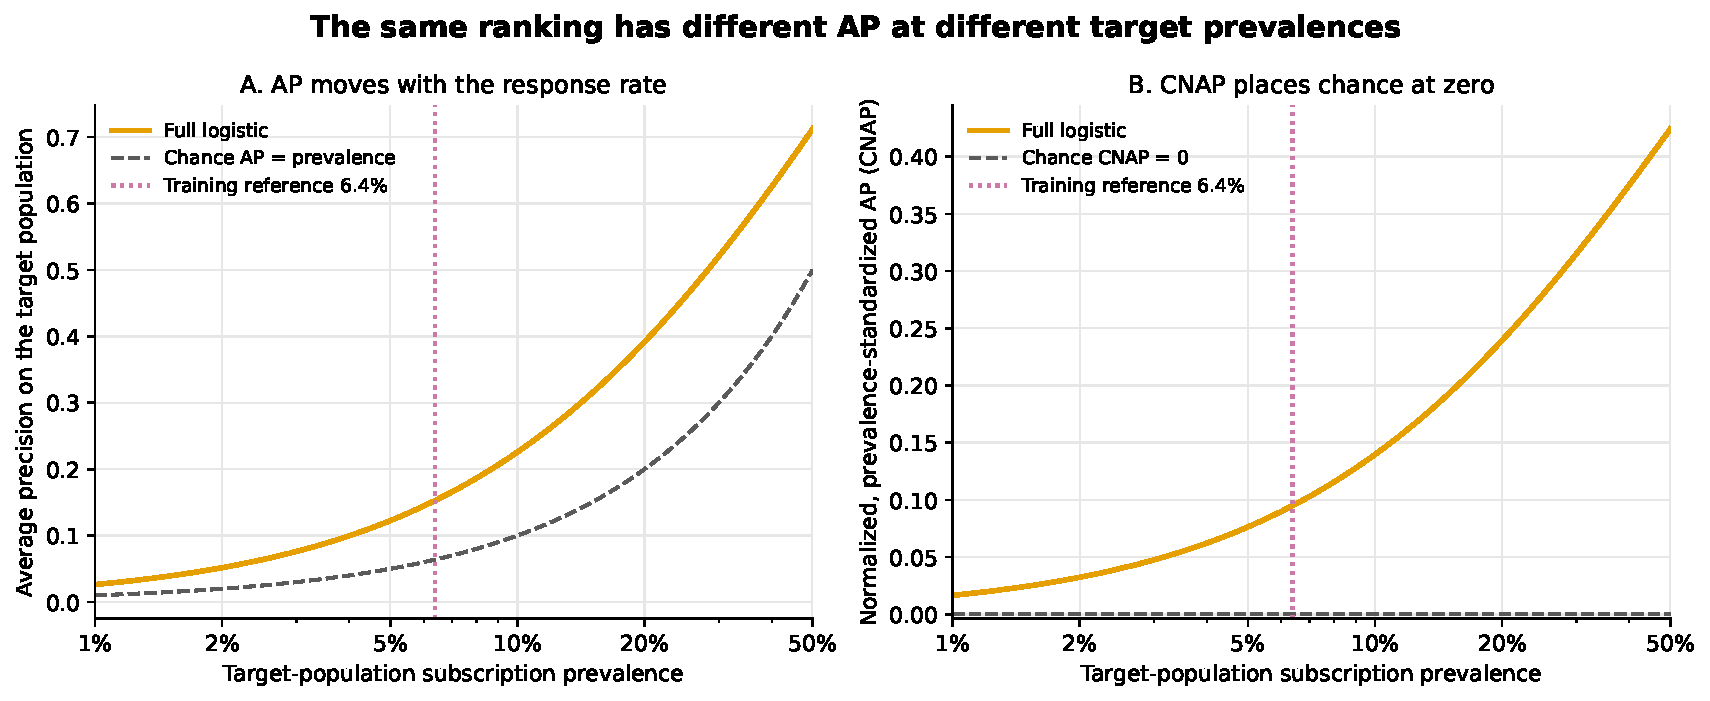
\includegraphics[width=\textwidth]{manuscript_images/banking-ap-target-prevalence.pdf}
\caption{Prior-standardized AP and CNAP for one fitted ranking across the
declared target-prevalence interval. The training prevalence is shown only as
a reference. Varying prevalence holds the observed class-conditional score
behavior fixed.}
\label{fig:bank-ap-cnap}
\end{figure}

The paired model difference is therefore formed before the weakest prevalence
is selected.
Figure~\ref{fig:bank-paired-profile} shows that the random-forest ordering
changes relative to full logistic regression inside the declared interval,
whereas the positive-control difference remains positive throughout.

\begin{figure}[htbp]
\centering
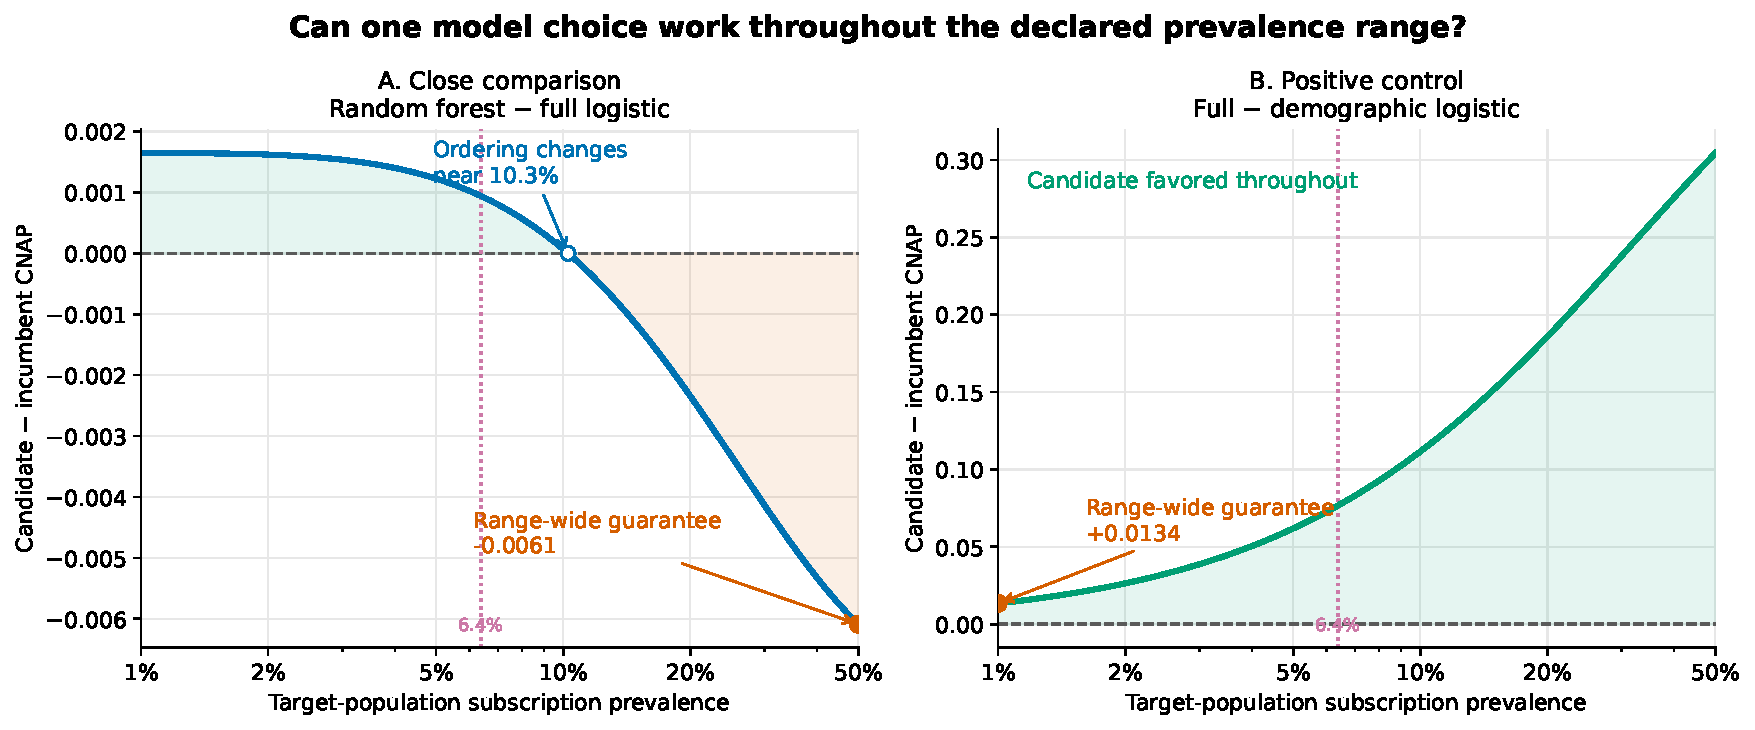
\includegraphics[width=\textwidth]{manuscript_images/banking-paired-prevalence-profile.pdf}
\caption{Paired CNAP differences in the temporal empirical evaluation. Panel A
compares random forest with full logistic regression; Panel B compares full
logistic regression with the demographic-only logistic model. Each orange
point is the infimum over the complete declared prevalence interval. The
limiting prevalence may differ between comparisons and orientations.}
\label{fig:bank-paired-profile}
\end{figure}
\clearpage

The temporal holdout forces $M=1$ and $K_E=1$. Random forest minus full
logistic regression had observed retained effect $-0.00609$; the reversed
orientation had retained effect $-0.00164$. Both fail the observed gate, so
anchor domination makes a full anchored verdict impossible. The construction
therefore stops at Stage 1: no computational AP collection is generated for
this comparison.

The positive control had observed retained effect $0.01341$; its reverse
retained effect was $-0.30442$. The forward orientation therefore passed the
observed gate for the single evaluation. We then used
$J=600$ paired computational replications stratified by outcome class, preserving the
observed evaluation counts of 2,540 subscribers and 5,698 non-subscribers. The
same resampled units were used for both models and throughout the prevalence
profile.

For the positive control, observed-anchored order-2 support was $0.01262$.
All 600 computational retained effects and the observed anchor cleared zero,
so anchored literal survival was $1.000$. The comparison passed Stage 2 and
supported replacement under the full one-evaluation assessment. The
unanchored order-2 projection was $0.01295$; its slightly larger value is
reported only to show the effect of retaining the observed anchor. The reverse
orientation returned no verdict.

This example establishes computational survival conditional on one temporal
evaluation. It records no survival across several empirical evaluations.

The corresponding observed-anchored AUROC case-mix analysis is reported in
Appendix~\ref{app:auroc-illustrations}. It uses the same temporal holdout and
paired model comparisons but challenges within-class composition rather than
target prevalence.

\subsection{Several empirical evaluations: ProteinGym}
\label{sec:proteingym-illustration}

ProteinGym organizes its deep-mutational-scanning (DMS) benchmark into
standardized assay-indexed datasets containing experimentally measured effects
for variants of a target protein or domain under a particular experimental
readout and context, together with released prediction scores
\cite{notin2023proteingym}. The task here is to rank single substitutions so
that experimentally deleterious or nonfunctional variants appear ahead of
functional variants. Such rankings can prioritize substitutions for further
interpretation or experimental study when exhaustive measurement is
unavailable.

We compared released zero-shot scores from three methodologically distinct
protein sequence models: the EVE ensemble evolutionary model, the ESM-1v
ensemble protein language model, and the ESM-2 650M protein language model
\cite{frazer2021eve,meier2021esm1v,lin2023esm2}. The comparisons were ESM-1v
ensemble against EVE ensemble, ESM-2 650M against ESM-1v ensemble, and ESM-2
650M against EVE ensemble. No model was fit or tuned for this study. The
replacement question was whether one released ranking retained a positive
advantage throughout the target deleterious-prevalence interval and across a
sufficiently large fraction of the admitted datasets.

We treated each retained assay-indexed dataset as one empirical evaluation.
Within a dataset, the substitutions supplied the paired model scores and
experimental labels used to compare the rankings; they were observations
within an evaluation, not separate empirical replications. This operational
choice preserves the standardized units supplied by ProteinGym and prevents
datasets containing more substitutions from dominating, but it does not claim
that an assay row is the uniquely correct or a statistically independent unit
of scientific replication. The across-evaluation challenge therefore asked
whether the average advantage recurred across these dataset contexts. Greater
domain knowledge could motivate another prospectively declared
operationalization---for example, grouping assays by protein, publication,
experimental system, or shared measurement context---which could change both
the effective collection size and the interpretation of across-evaluation
support.

We used ProteinGym version 1.3 substitution data, retained assays with manual
biological cutoffs, and retained single amino-acid substitutions.
Experimentally nonfunctional or deleterious variants formed the positive class.
Because the released scores were oriented toward predicted fitness, they were
negated so that larger analyzed values represented stronger predicted
deleteriousness. The aligned cohort contained 277,873 substitutions in 91
assays, including 96,987 deleterious and 180,886 functional variants.

The observed deleterious fraction ranged from $0.025$ to $0.869$ across assays,
with median $0.315$ and interquartile range $[0.244,0.440]$. All 91 assay
fractions lay within the declared target interval $[0.01,0.90]$. The pooled
fraction was $96{,}987/277{,}873=0.349$, but this value weights assays by their
numbers of retained substitutions and is not the prevalence of a typical
assay.

Ordinary empirical AP would evaluate each ranking at the deleterious fraction
observed in that assay. Prior standardization instead evaluates every assay
over the common target interval while retaining that assay's observed joint
class-conditional score behavior. It changes only the target class prior; each assay's observed within-class
score behavior and its protein, measurement process, and experimental context
are preserved.

Within each assay, the paired CNAP difference was evaluated throughout the
complete interval and its smallest value was retained as the observed anchor.
A positive anchor therefore means that the candidate exceeded the incumbent at
every declared target prevalence in that assay. Figure~\ref{fig:proteingym-effects}
shows positive and negative anchors in every comparison, so the relative model
ordering was not stable across the admitted assays.

\begin{figure}[htbp]
\centering
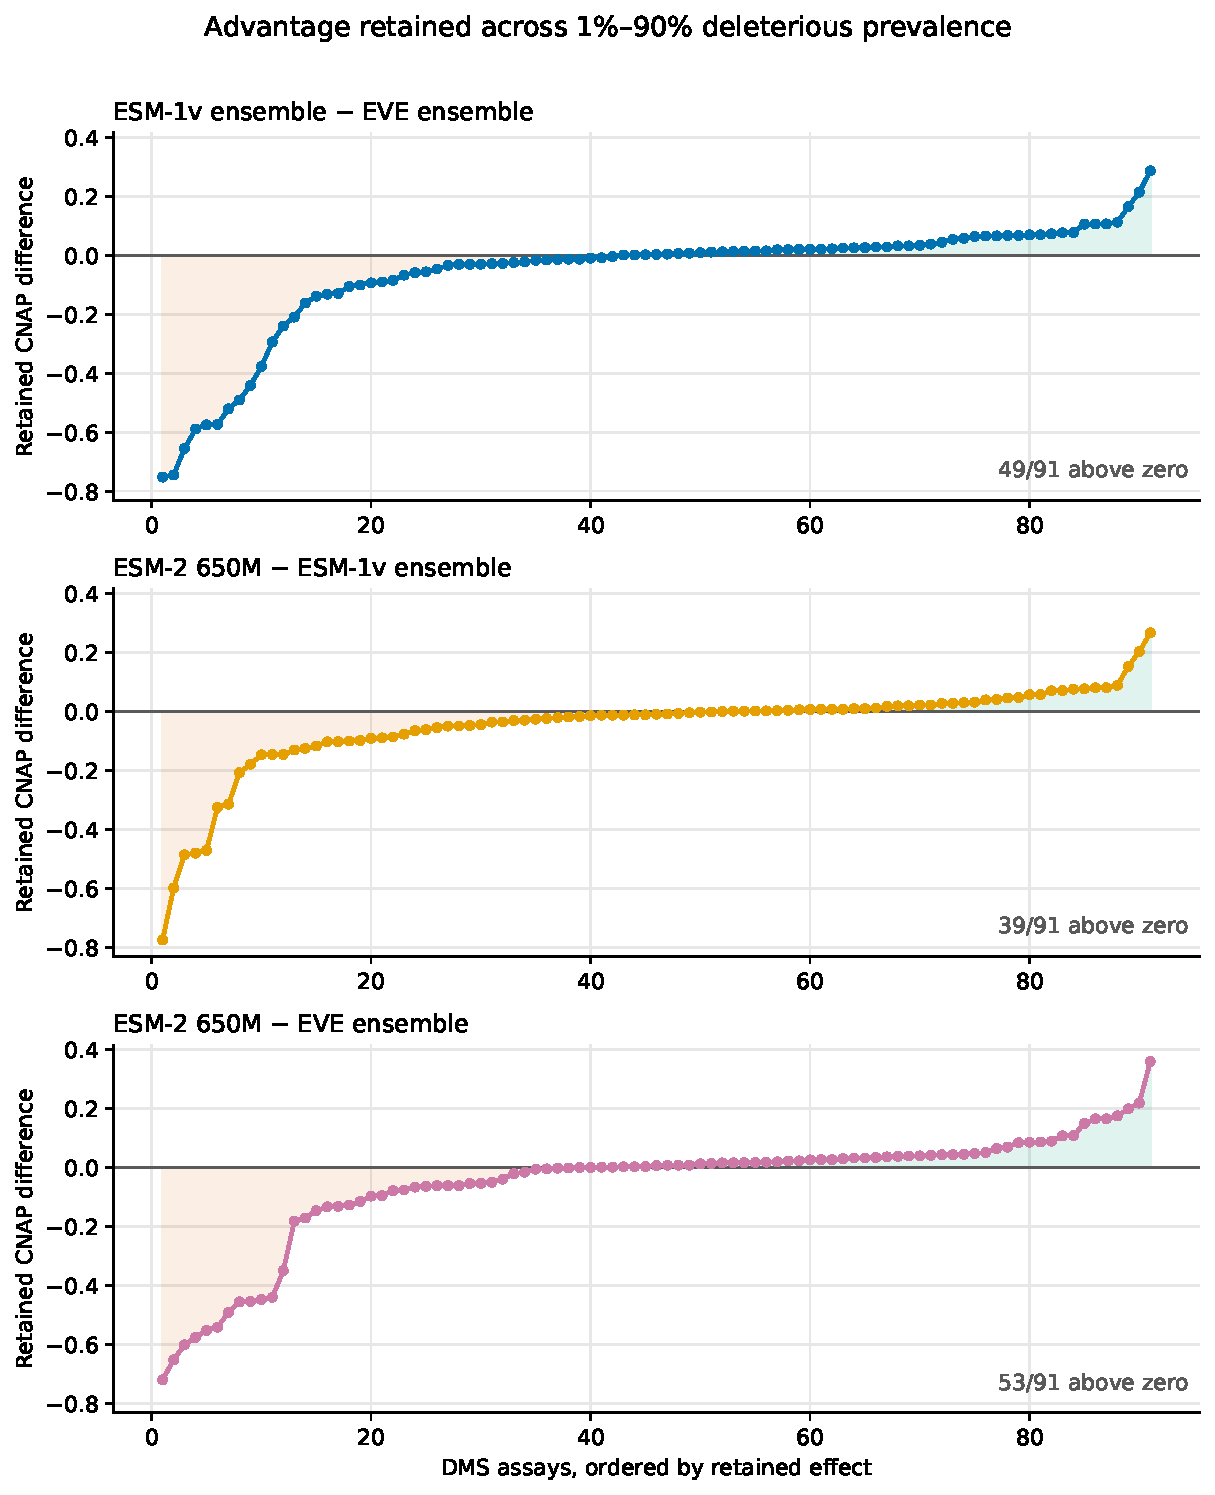
\includegraphics[width=0.94\textwidth]{manuscript_images/proteingym-observed-assay-effects.pdf}
\caption{Observed retained assay effects for the three ProteinGym comparisons
over the 1\%--90\% target-prevalence interval. Each point is one complete DMS
assay after its paired difference has faced the full interval. Panels order
assays separately; the horizontal position does not identify the same assay
between panels.}
\label{fig:proteingym-effects}
\end{figure}

Table~\ref{tab:proteingym-results} reports the Stage 1 challenge across the 91
assay anchors. With $K_E=2$, each complete empirical challenge contains two
distinct assays and survives the floor $d=0$ only when both anchors are
positive.

\begin{table}[htbp]
\centering
\caption{Stage 1 observed order-2 ProteinGym results. All comparisons use the
same 91 assays and policy.}
\label{tab:proteingym-results}
\begin{tabularx}{\textwidth}{@{}Xrrrr@{}}
\toprule
Candidate minus incumbent & Support & Assays $>0$ & Pair survival & Gate \\
\midrule
ESM-1v ensemble minus EVE ensemble & $-0.1548$ & $49/91$ & $0.287$ & Fail \\
ESM-2 650M minus ESM-1v ensemble & $-0.1175$ & $39/91$ & $0.181$ & Fail \\
ESM-2 650M minus EVE ensemble & $-0.1556$ & $53/91$ & $0.337$ & Fail \\
\bottomrule
\end{tabularx}
\end{table}

An order-2 pair contains two complete assay evaluations, not two protein
variants. There are $\binom{91}{2}=4{,}095$ such pairs, and a pair survives at
$d=0$ only when both assay anchors are positive. The strict requirement
$\psi_{2,0}>0.81$ requires at least 82 of 91 assays to clear zero because
$\binom{82}{2}/\binom{91}{2}=0.811>0.81$. Thus more than 81\% of all distinct
assay pairs survive only if at least 82 of 91 individual assays---just over
90\%---retain a positive range-wide advantage. None approached that count.

\begin{figure}[htbp]
\centering
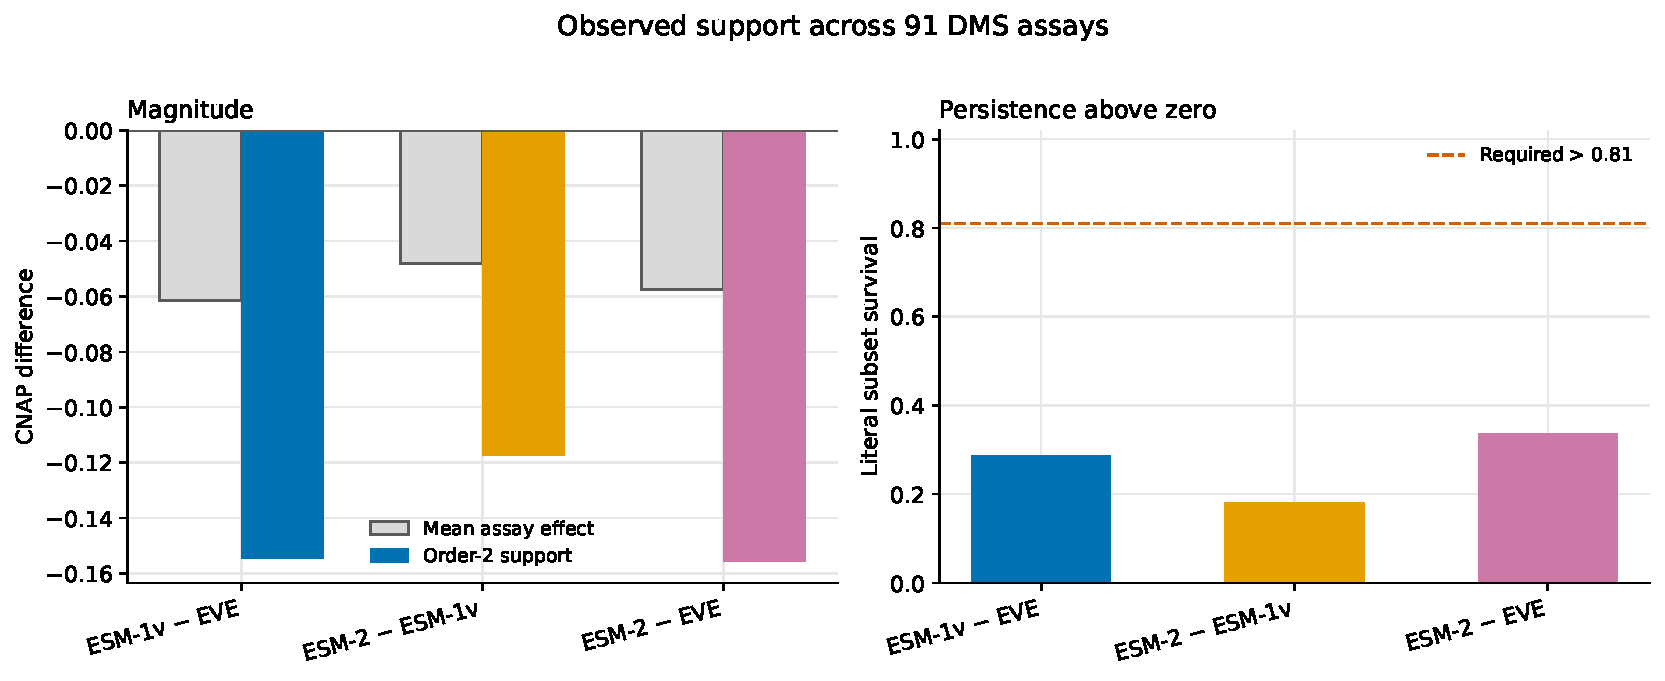
\includegraphics[width=\textwidth]{manuscript_images/proteingym-two-part-decision.pdf}
\caption{Observed mean assay effect, order-2 support, and literal assay-pair
survival for the three ProteinGym comparisons. The left panel shows how the
noncompensating order-2 challenge moves magnitude below the assay mean. The
bars on the right are exact fractions of the 4,095 assay pairs whose two
anchors both exceed zero.}
\label{fig:proteingym-decision}
\end{figure}

All forward and reverse comparisons fail the empirical gate. This does not show
that an incumbent was superior in every assay or that the compared models were
equivalent. It shows that no examined orientation produced a positive
range-wide advantage in enough assay evaluations to satisfy the declared
replacement policy.

Because the observed assay anchors fail the necessary gate, resampling
substitutions within assays could not support replacement under the anchored
rule. Such resampling might describe sensitivity to the represented
substitutions, but it could neither convert an observed assay failure into a
success nor add new proteins, assays, laboratories, or measurement mechanisms.
We therefore do not resample merely to fill the interior $M>1,K_C>0$ case.
Doing so would also require a defensible account of within-assay dependence,
protein-position clustering, sparse outcomes, and the scientific identity of
the resampling unit.

The 91 assay-indexed datasets represent 80 UniProt proteins and 60
publications. Twenty assay rows share a protein with another retained assay,
and 42 come from publications contributing more than one assay. We retained
these multiplicities in the finite collection rather than grouping by protein
or publication. Under the declared assay-level regime, target interval,
empirical order, and policy thresholds, none of the examined orientations
supports model replacement. The result concerns the 91 admitted assay
evaluations; it does not establish global model superiority or estimate
performance in an unseen assay.

Appendix~\ref{app:auroc-illustrations} also reports the observed-only AUROC
boundary for these same 91 assays. Because every declared comparison fails
that empirical gate, no within-assay computational AUROC collection is
generated.


\section{Interpretation, reporting, and scope}
\label{sec:discussion}

\subsection{What the quantities support}

Observed support describes what the admitted empirical evaluations retain
after the condition challenge. Anchored empirical--computational support
describes what remains when each selected empirical evaluation retains both
its observed anchor and selected computational effects. Neither is a portable
property of a model. Both are indexed by the orientation, condition set,
evaluation regime, challenge orders, and---for the full construction---the
computational procedure.

The hierarchy is falsification-oriented. It asks how much of a claim remains
after named opportunities for failure have been imposed. Passing means that the
claim survived those attempted refutations. It does not establish truth beyond
them \cite{popper1959logic,popper1963conjectures}. In particular, the finite
empirical list is not treated as a random sample from a latent population of
evaluations, and the nested survival fraction is not a confidence level or an
estimate of future replication probability.

Computational replication deepens but does not broaden the empirical basis.
Increasing $M$ adds empirical tests. Increasing $J_m$ improves numerical
approximation. Increasing $K_E$ or $K_C$ strengthens a declared challenge.
These actions answer different questions and should not share the generic label
``more replications.''

The result remains a ranking-performance claim. Calibration, utility, resource
constraints, and consequences of acting on selected cases may determine a
deployment decision but are not evaluated by the replacement rule.

\subsection{Relation to population robustness and inference}
\label{sec:related-frameworks}

Some operations have analogues in frameworks that begin with a population
probability law. Shared algebra does not supply a shared interpretation.

The retained effect $\inf_{c\in\CSet}\Delta_c(D)$ resembles an intersection
bound. Intersection-bound inference instead concerns infima or suprema of
population-indexed functions and their repeated-sampling behavior
\cite{chernozhukov2013intersection}. Here the infimum extracts the exact uniform
lower level of a condition profile computed in one complete finite evaluation.

The ordered finite-list form of $-S_K$ resembles a spectral loss functional
\cite{acerbi2002spectral}, and the survival integral resembles a distortion or
Choquet representation \cite{wang1996premium}. In those settings, order
statistics commonly estimate a functional of a random quantity. Here the
representations are exact identities for a declared finite indexed list or
array. No superpopulation interpretation is imported.

The empirical case-mix sets developed in Appendix~\ref{app:auroc} resemble
ambiguity sets in distributionally robust optimization
\cite{shapiro2017distributionally,bental2013robust}. Their concentration factor
is a deterministic allowance over represented cases, not a confidence radius
around an unknown distribution. Population coverage results from data-driven
robust optimization require a different inferential target and assumptions
\cite{duchi2021statistics}.

Probability is used here when a target population description or deliberately
constructed randomization requires it. The target prevalence describes a
counterfactual population composition. The resampling law defines a
computational projection. The exchangeable-label law defines a reference
diagnostic. None is silently promoted into a law generating unseen empirical
evaluations.

Inferential comparisons of classifiers across repeated train--test samples or
multiple benchmark datasets instead ask whether performance differences
generalize under sampling assumptions
\cite{nadeau2003inference,bouckaert2004estimating,demsar2006statistical}. The
empirical subset average here is an exact finite selection over admitted
evaluations and supplies no sampling law for unseen datasets.

\subsection{Minimum reporting content}

A concise report should identify the claim and the stage at which it survived
or failed.

\begin{table}[htbp]
\centering
\caption{Minimum reporting content for an anchored replacement analysis.}
\label{tab:reporting}
\begin{tabularx}{\textwidth}{@{}>{\raggedright\arraybackslash}p{0.22\textwidth}>{\raggedright\arraybackslash}X@{}}
\toprule
Component & Report \\
\midrule
Claim and policy & Candidate and incumbent orientation; $\delta,d,\gamma$; reverse orientation; final verdict and whether it refers to the full or reduced assessment \\
Condition and effect & $\CSet$ and its basis; transport commitments; paired construction; tie convention; numerical condition search and tolerance \\
Empirical evidence & $\Regime$; admission and evaluation unit; contexts; known dependence or multiplicity; pooling and empirical selection rule; $M$ and $N_m$; observed anchors; $K_E$; observed support and survival; number of anchors clearing $d$ \\
Computational challenge & $\Boot$ and resampling unit; pairing and dependence preservation; $J_m$; $K_C$; whether row selections are independent; anchored support and survival; row survival fractions \\
Diagnostics & Binding anchors; computational effects below their anchors; values near $d$; seed and $J_m$ stability; sensitivity to prespecified alternative orders, conditions, and floors \\
Scope & Represented case types and contexts; absent mechanisms; whether a reference randomization is asserted; external premise required for deployment \\
\bottomrule
\end{tabularx}
\end{table}

A headline statement may read:
\begin{quote}
Across $M$ admitted empirical evaluations satisfying the declared
regime, direct order-$K_E$ observed support was [value] and observed literal
survival above $d=[\text{value}]$ was [value], so the comparison
[passed/failed] the empirical gate. [If passed:] Each evaluation was then
challenged using $J_m$ paired computational replications under the declared
procedure. With computational order $K_C$, observed-anchored nested support was
[value] and nested literal survival was [value]. The full assessment therefore
returned [supported replacement/no verdict] under $\delta=[\text{value}]$ and
$\gamma=[\text{value}]$. The computational layer recombines represented units;
it adds no empirical evaluations or unrepresented failure mechanisms.
\end{quote}
If the gate fails, the report should state that anchor domination makes passage
of the full rule impossible and that computation was unnecessary for the
verdict. If Stage 2 was not declared, any passing verdict should be labeled
support under the reduced observed-only assessment.

\subsection{Limits and transport commitments}

Prior standardization varies the class prior while retaining observed joint
class-conditional score behavior. It does not address changes within outcome
class. Computational resampling recombines represented units. It does not
extrapolate to absent units. Additional empirical reach requires additional
evaluations within $\Regime$, not stronger probabilistic language about the
evaluations already observed.

Tie averaging removes expected credit for outcome-blind refinement within
score blocks. It does not create full label exchangeability. Matched,
clustered, and heterogeneous-risk designs may retain design-specific reference
anchors.

Anchoring deliberately keeps the effect actually obtained in a finite
empirical evaluation binding. An unusually adverse anchor remains binding even
when most resamples are favorable. This is not treated as bias to be corrected:
the computational distribution may expose or describe fragility, but it does
not erase the empirical test.

The choices of $\CSet$, $\Regime$, $\Boot$, $K_E$, and $K_C$ remain
scientific commitments. Widening the condition set or increasing an order
mechanically strengthens a fixed challenge, but no such operation proves that
the assessment contains the failures most relevant to deployment.

\subsection{Beyond AP}

The hierarchy accepts any observed and computational retained effects of the
form
\[
z_m^{\mathrm{obs}}=\inf_{c\in\CSet}\Delta_c(D_m),
\qquad
z_{mj}^{\mathrm{comp}}=\inf_{c\in\CSet}\Delta_c(D_m^{(j)}).
\]
Pure prior shift supplies no AUROC challenge. AUROC depends on the two
class-conditional score distributions rather than the class prior.
Appendix~\ref{app:auroc} instead uses capped within-class empirical
redistributions as the condition-level challenge. The order remains: optimize
the case-mix condition within each full empirical or computational evaluation.
Complete nested challenges then jointly select empirical rows and within-row
computational subsets, retain every selected row's observed anchor, and take
the minimum over each complete nested selection before any averaging occurs.


\section{Conclusion}

A replacement claim becomes stronger only when the attempted refutations it
has survived are made explicit. For AP, the first challenge is a declared set
of target prevalences. For empirical persistence, it is a set of evaluations
admitted by a regime under a declared selection rule; only those meeting the
stronger separation conditions are empirical replications. For dependence on
the represented units, the assessment may include a scientifically defensible
computational resampling procedure. These levels can be combined without
treating them as exchangeable.

The construction first pairs the models, resolves outcome-blind tie refinement,
and retains the weakest advantage over target prevalence in every complete
observed or computational evaluation. It then preserves empirical identity:
each selected row keeps its observed retained effect as a mandatory anchor and
adds selected computational effects as further opportunities for failure. The
complete nested challenge is formed before its weakest effect is averaged with
the minima of other challenges.

Observed anchoring gives the direct empirical analysis a precise role. Direct
observed support and literal survival form a necessary gate. Failure there
proves that the full anchored rule cannot pass. A claim that clears the gate
proceeds to the computational challenge, where computation may preserve or
reduce the credited support but cannot overwrite the evidence actually
obtained.

Supported magnitude and literal survival remain two summaries of the same
objects:
\[
\Sanc_{K_E;K_C}
=
a+\int_a^b\Psianc_{K_E;K_C,s}\,ds.
\]
The first retains the size of every complete challenge minimum. The second
records the fraction clearing a declared floor. A finite-evidence replacement
rule requires both to meet prespecified standards, first at the empirical gate
and then, when declared, under the full hierarchy.

The illustrations show the two stopping points. The Bank Marketing positive
control passes its observed gate and then its anchored computational challenge;
the closer comparison fails at the gate. The ProteinGym comparisons fail
across observed assays, so computational perturbation is unnecessary for their
verdicts. In neither setting does computation manufacture empirical reach.

The central claim is consequently limited but operational: computational
replication can deepen the challenge applied to each empirical evaluation, but
it cannot increase the number of empirical evaluations, erase an observed
effect, or reveal a failure mechanism that the empirical evidence never
contained.


\appendix

\section{Empirical prior-standardized average precision}
\label{app:ap}

\subsection{Definition and weighted implementation}

Let
\[
D=\{(s_i,y_i)\}_{i=1}^N,
\qquad y_i\in\{0,1\},
\]
with positive and negative counts $N_+=\sum_i y_i>0$ and
$N_-=N-N_+>0$. Let $c_1>\cdots>c_H$ be the distinct score values. At
threshold $h$, define
\[
\operatorname{TP}_h
=\sum_i\mathbf 1\{y_i=1,s_i\geq c_h\},
\qquad
\operatorname{FP}_h
=\sum_i\mathbf 1\{y_i=0,s_i\geq c_h\},
\]
and
\[
r_h=\frac{\operatorname{TP}_h}{N_+},
\qquad
f_h=\frac{\operatorname{FP}_h}{N_-}.
\]
With $r_0=0$, noninterpolated prior-standardized AP under the threshold-block
convention is
\begin{equation}
\AP_\pi(D)
=
\sum_{h=1}^H
(r_h-r_{h-1})
\frac{\pi r_h}{\pi r_h+(1-\pi)f_h}.
\label{eq:empirical-ap}
\end{equation}
All units sharing a score enter one block. A negative-only block has no recall
increment, but its false positives reduce precision in later blocks.

The same quantity follows by weighting each positive unit by $\pi/N_+$ and
each negative unit by $(1-\pi)/N_-$. Weighted precision at threshold $h$ is
the fraction in Equation~\eqref{eq:empirical-ap}, while weighted recall remains
$r_h$.

\subsection{Behavior across prevalence}

Combining Equations~\eqref{eq:cnap} and \eqref{eq:empirical-ap} gives
\begin{equation}
\CNAP_\pi(D)
=
\sum_{h=1}^H
(r_h-r_{h-1})
\frac{\pi(r_h-f_h)}
{\pi r_h+(1-\pi)f_h}.
\label{eq:cnap-profile}
\end{equation}
The derivative of one threshold contribution is
\begin{equation}
\frac{\partial}{\partial\pi}
\left\{
\frac{\pi(r_h-f_h)}
{\pi r_h+(1-\pi)f_h}
\right\}
=
\frac{f_h(r_h-f_h)}
{\{\pi r_h+(1-\pi)f_h\}^2}.
\label{eq:cnap-derivative}
\end{equation}
If $r_h\geq f_h$ at every threshold with positive recall increment, the
marginal profile is nondecreasing. A paired difference may remain nonmonotone
even when both marginal profiles are nondecreasing.


\section{Properties of finite-list and nested support}
\label{app:support-proofs}

\subsection{Finite-list survival and ordered representations}

For $\mathbf t=(t_1,\ldots,t_L)$ with entries in $[a,b]$, let
\[
R_s=\sum_{\ell=1}^L\mathbf 1\{t_\ell>s\}.
\]
For each $I\in\mathcal I_{L,K}$,
\[
\min_{\ell\in I}t_\ell
=
a+\int_a^b
\mathbf 1\{t_\ell>s\text{ for every }\ell\in I\}\,ds.
\]
Exactly $\binom{R_s}{K}$ subsets have every effect above $s$. Averaging gives
\begin{equation}
S_K(\mathbf t)
=
a+\int_a^b
\frac{\binom{R_s}{K}}{\binom{L}{K}}\,ds.
\label{eq:finite-survival}
\end{equation}
Thus finite-list literal survival at floor $d$ is
\begin{equation}
\psi_{K,d}(\mathbf t)
=
\frac{\binom{R_d}{K}}{\binom{L}{K}}.
\label{eq:finite-literal}
\end{equation}

Let $t_{(1)}\leq\cdots\leq t_{(L)}$. The minimum of exactly
$\binom{L-i}{K-1}$ distinct order-$K$ subsets is $t_{(i)}$. Hence
\begin{equation}
S_K(\mathbf t)
=
\binom{L}{K}^{-1}
\sum_{i=1}^{L-K+1}
\binom{L-i}{K-1}t_{(i)}.
\label{eq:finite-ordered}
\end{equation}
This is an exact identity for the indexed finite list, not an estimate of a
population spectral functional.

\subsection{Proof of the nested magnitude--survival identity}

Apply the layer-cake identity to each complete challenge value $t$:
\[
t
=
a+\int_a^b\mathbf 1\{t>s\}\,ds.
\]
The challenge clears $s$ exactly when, for every selected row, its observed
anchor clears $s$ and every selected computational effect clears $s$.

Conditional on row $m$, the fraction of computational selections having that
property is $q^{\mathrm{anc}}_{m,K_C,s}$. Under independent row selections, the
fraction for empirical subset $I$ is their product. Averaging over empirical
subsets gives Equation~\eqref{eq:anchored-survival}. Averaging the layer-cake
identity over all complete challenges and interchanging the finite average and
integral proves Equation~\eqref{eq:nested-survival-identity}.

For coordinated row selections, replace the product by the survival
probability under their declared joint selection law. The layer-cake identity
continues to hold for that direct challenge definition.

\subsection{Boundary reduction and anchor domination}

Under $K_C=0$, the empty computational minimum is $+\infty$. Therefore
the contribution from row $m$ is
$\min\{z_m^{\mathrm{obs}},+\infty\}=z_m^{\mathrm{obs}}$, and the average over
empirical subsets is precisely $S_{K_E}(\mathbf z^{\mathrm{obs}})$. The
corresponding complete challenge clears $d$ precisely when all selected
observed anchors clear it, giving Equation~\eqref{eq:observed-boundary}.

For every complete nested selection,
\[
\min_{m\in I}
\left\{z_m^{\mathrm{obs}},
\min_{j\in A_m}z_{mj}^{\mathrm{comp}}\right\}
\leq
\min_{m\in I}z_m^{\mathrm{obs}}.
\]
Averaging proves Equation~\eqref{eq:magnitude-domination}. If a complete
nested selection clears $d$, its selected observed anchors necessarily clear
$d$. The set of surviving nested selections is consequently contained in the
set permitted by the observed anchors, proving
Equation~\eqref{eq:survival-domination}.

Removing the mandatory anchors replaces every selection minimum by a value no
smaller than its anchored counterpart. The analogous domination of the
unanchored nested projection follows for magnitude and survival.

\subsection{Proof of hierarchical challenge monotonicity}

Enlarging $\CSet$ lowers or preserves every observed and computational retained
effect. Both anchored magnitude and literal survival are coordinatewise
nondecreasing functions of those entries, so neither quantity can increase
under the enlarged condition challenge.

For the computational order, every order-$K_C+1$ subset contains
$K_C+1$ order-$K_C$ subsets. Its anchored minimum is no larger than the
average of their anchored minima. Averaging over all order-$K_C+1$ subsets
counts every order-$K_C$ subset the same number of times. This proves
within-row monotonicity. Applying the same argument simultaneously within the
selected rows and then averaging across empirical subsets proves monotonicity
of the full supported magnitude.

At a fixed floor, a surviving order-$K_C+1$ computational subset has all of
its order-$K_C$ subsets surviving. Equivalently,
\[
\frac{\binom{R}{K_C+1}}{\binom{J}{K_C+1}}
\leq
\frac{\binom{R}{K_C}}{\binom{J}{K_C}}
\]
for $0\leq R\leq J$. Thus every row survival fraction is nonincreasing in
$K_C$.

The same subset-counting argument across empirical rows proves magnitude
monotonicity in $K_E$. For survival, couple an order-$K_E+1$ empirical subset
with a uniformly selected order-$K_E$ subset inside it. The product of row
survival fractions in $[0,1]$ cannot decrease when a factor is removed.
Averaging the coupling proves monotonicity in $K_E$.

\subsection{Proof of the nested orientation bound}

For each full empirical or computational evaluation $e$, write
\[
L_e=\inf_{c\in\CSet}\Delta_c^{A:B}(D_e),
\qquad
U_e=\sup_{c\in\CSet}\Delta_c^{A:B}(D_e).
\]
The retained effect in the reverse orientation is $-U_e$. For a fixed nested
selection $Q$ of observed anchors and computational entries, the forward and
reverse challenge values are
\[
\min_{e\in Q}L_e
\qquad\text{and}\qquad
-\max_{e\in Q}U_e.
\]
Because $L_e\leq U_e$ for every entry,
\[
\min_{e\in Q}L_e-\max_{e\in Q}U_e\leq0.
\]
Averaging over the same nested selections proves
Equation~\eqref{eq:orientation}.

\subsection{Noncomposition and preservation of index identity}

For profiles $U_c$ and $V_c$, define
\[
U_\CSet=\inf_cU_c,
\qquad
V_\CSet=\inf_cV_c,
\qquad
T_\CSet=\inf_c(U_c-V_c).
\]
Choosing a condition that approaches the infimum of $U$ gives
$T_\CSet\leq U_\CSet-V_\CSet$. Thus separately challenged marginal model
effects dominate the correctly paired retained effect cellwise. Coordinatewise
monotonicity propagates that discrepancy through the anchored hierarchy.

Row-summary composition fails because the minimum is concave. For independent
row selections $A_1,\ldots,A_M$,
\[
\E\!\left[
\min_{m\in I}
\left\{
z_m^{\mathrm{obs}},
\min_{j\in A_m}z_{mj}^{\mathrm{comp}}
\right\}
\right]
\leq
\min_{m\in I}
\E\!\left[
\min\left\{
z_m^{\mathrm{obs}},
\min_{j\in A_m}z_{mj}^{\mathrm{comp}}
\right\}
\right].
\]
The left side is the complete-challenge construction; the right side is what a
row-first summary uses before the outer minimum. Strict inequality occurs in
the running example.

Flattening can fail even more fundamentally. Suppose one empirical row has
anchor $1$ and all computational effects $1$, while a second row has anchor
$-1$ and all computational effects $-1$. The observed order-1 support is zero,
regardless of the Monte Carlo counts. A flattened mean becomes
$(J_1-J_2)/(J_1+J_2)$ and may approach either endpoint merely by allocating
more draws to one row. The flattened list therefore responds to approximation
counts as though they were empirical evidence. Preserving the row index avoids
that change of scientific meaning.


\section{Tie averaging and paired reference properties}
\label{app:paired-proofs}

\subsection{Why ordinary pairing rewards arbitrary refinement}

Take four units with two positive and two negative labels at $\pi=1/2$.
Model $A$ assigns four distinct scores and model $B$ assigns one common score.
Assign the labels uniformly over the six possible arrangements. Neither score
vector contains outcome information. Under ordinary stepwise AP, model $A$ has
expected AP $49/72$, while model $B$ has AP $1/2$ under every assignment.
Therefore
\[
\E[\CNAP_A-\CNAP_B]=\frac{13}{36}.
\]
For two independently randomized label assignments, the expected order-2
minimum of the paired differences remains positive at $29/216$. Pairing has
favored the model that broke ties without information.

An additive reference correction cannot remove this displacement at every
performance level. The randomization displacement is positive near no
association but vanishes at perfect separation, where both models reach the
ceiling. Refinement neutrality is therefore obtained only when outcome-blind
tie handling occurs before condition and replication minima are applied.

\subsection{Proof of refinement neutrality}

Condition on $S_B$ and $Y$. Under Proposition~\ref{prop:refinement}, model
$A$'s strict ranking $O_A$ is uniform on the rankings consistent with $S_B$.
Tie-averaged AP for $A$ is the conditional expectation of ordinary AP over
whatever ties $A$ retains. By the tower property,
\[
\E[\APta_{A,\pi}\mid S_B,Y]
=
\E[\AP_\pi(D_{O_A})\mid S_B,Y].
\]
Uniformity of $O_A$ turns the right side into the average of ordinary AP over
all strict rankings consistent with $S_B$, which is $\APta_{B,\pi}$.

\subsection{Exchangeable-label reference behavior}

\begin{definition}[Exchangeable-label reference law]
Conditionally on both score vectors and the positive count in each observed
evaluation, every label vector with that count has equal probability. After a
label vector is assigned, $\Boot$ is applied conditionally to that randomized
evaluation, preserving pairing and the declared resampling structure.
\end{definition}

Fix $N_+$, $N_-$, and a strict ranking. Under full exchangeability, the label
sequence read along the ranking is uniform over all $\binom N{N_+}$ sequences
with $N_+$ positives. Reading labels along any other strict ranking is a
bijection of the same sequences. Expected tie-averaged CNAP therefore depends
on the class counts and $\pi$, but not on the fixed score vector or its tie
structure. Hence
\begin{equation}
\E_0[\Delta^{A:B}_\pi(D_m)]=0
\label{eq:reference-cell}
\end{equation}
for every condition-specific observed paired effect.

Because
\[
\E_0\!\left[
\inf_{\pi\in\PSet}\Delta^{A:B}_\pi(D_m)
\right]
\leq
\inf_{\pi\in\PSet}
\E_0[\Delta^{A:B}_\pi(D_m)]
=0,
\]
the expected observed retained anchor is nonpositive. Anchor domination gives
\[
\Thetaanc_{A:B;K_E,K_C}
\leq
S_{K_E}(\mathbf z^{A:B,\mathrm{obs}})
\leq
\frac1M\sum_{m=1}^Mz_m^{A:B,\mathrm{obs}}.
\]
Taking reference expectation proves that expected anchored support is
nonpositive. Exchanging the model orientation proves the same result for
$B:A$. This proof keeps the observed labels and the computational procedure in
their proper order: labels are randomized within each empirical evaluation,
then $\Boot$ is applied conditionally to that randomized evaluation.

Full exchangeability is stronger than independence. Take four units in two
matched pairs, each constrained to contain one positive. Let model $A$ tie all
units, while model $B$ places the first pair above the second and ties within
pairs. At $\pi=1/2$, exact tie averaging over the four design-permitted label
assignments yields $\CNAPta_A-\CNAPta_B=1/36$ in one orientation for every
assignment. Restricted symmetry divides rankings into different orbits; tie
averaging within blocks cannot move a ranking between them.

\subsection{Why paired null centering fails}

Take two positive and two negative units at $\pi=1/2$, with
\[
s_A=(4,3,2,1),
\qquad
s_B=(2,2,1,1),
\]
and let the two highest-scored units be positive. Both models separate the
classes perfectly, so every stratified empirical-resampling evaluation has
CNAP one for each model and paired difference zero.

Under joint label permutation, exact enumeration of unanchored order-2 support
gives expected value $35/384$ for $A-B$ and $-295/1152$ for $B-A$.
Subtracting these reference values would report a positive corrected value of
about $0.256$ for the second orientation, favoring the coarser model although
both predictions are perfect. The displacement is not an additive constant;
the reference law is therefore diagnostic rather than a centering correction.


\section{Closed-form computation of tie-averaged AP}
\label{app:tie-computation}

Index distinct score blocks by $h=1,\ldots,H$ from highest to lowest. Let block
$h$ contain $a_h$ positives and $b_h$ negatives, with $m_h=a_h+b_h$, and let
\[
A_h=\sum_{\ell<h}a_\ell,
\qquad
B_h=\sum_{\ell<h}b_\ell.
\]
Then
\begin{align}
\APta_\pi(D)
&=
\sum_{h=1}^H
\frac{a_h}{N_+}\frac1{m_h}
\sum_{k=1}^{m_h}
\sum_{t=\max(0,k-1-b_h)}^{\min(k-1,a_h-1)}
\frac{\binom{a_h-1}{t}\binom{b_h}{k-1-t}}
{\binom{m_h-1}{k-1}}
\notag\\
&\qquad\qquad\times
\frac{\pi r_{hkt}}
{\pi r_{hkt}+(1-\pi)f_{hkt}},
\label{eq:tie-closed}
\end{align}
where
\[
r_{hkt}=\frac{A_h+t+1}{N_+},
\qquad
f_{hkt}=\frac{B_h+k-1-t}{N_-}.
\]

To obtain the formula, fix one positive unit in block $h$. Under a uniformly
random ordering of the block, its position $k$ is uniform on
$\{1,\ldots,m_h\}$. Given $k$, the number $t$ of other positive units in the
$k-1$ preceding positions is hypergeometric with $a_h-1$ positives and $b_h$
negatives available. The last fraction is prior-standardized precision when
that positive enters the ranking. Averaging over $t$ and $k$, multiplying by
the $a_h$ positives in the block, and summing across blocks gives the result.

The calculation costs $O(\sum_hm_h^2)$ operations. Its combinatorial weights
do not depend on $\pi$ and can be reused throughout the prevalence search. When
all scores are distinct, Equation~\eqref{eq:tie-closed} reduces to ordinary
stepwise AP.


\section{Computation for several empirical evaluations}
\label{app:computation}

\subsection{Observed gate}

For each admitted empirical evaluation, compute
\[
z_m^{\mathrm{obs}}
=
\inf_{c\in\CSet}\Delta_c(D_m).
\]
Sort the anchors as
$z_{(1)}^{\mathrm{obs}}\leq\cdots\leq z_{(M)}^{\mathrm{obs}}$. Then
\begin{equation}
S_{K_E}(\mathbf z^{\mathrm{obs}})
=
\binom{M}{K_E}^{-1}
\sum_{i=1}^{M-K_E+1}
\binom{M-i}{K_E-1}z_{(i)}^{\mathrm{obs}}.
\label{eq:sorted-observed}
\end{equation}
Observed literal survival follows from the count of anchors above $d$. If the
gate fails, the primary algorithm stops.

\subsection{Finite-array sweep}

If the gate passes, generate each row's computational effects. Direct
enumeration requires considering
\[
\sum_{I\in\mathcal I_{M,K_E}}
\prod_{m\in I}\binom{J_m}{K_C}
\]
complete selections and quickly becomes infeasible. The survival
representation avoids this enumeration.

At each effect level $s$, compute the row fractions in
Equation~\eqref{eq:row-survival}, then evaluate the elementary symmetric
polynomial in Equation~\eqref{eq:elementary-symmetric}. Its recursion is
\begin{equation}
e_0^{(m)}=1,
\qquad
e_k^{(m)}
=
e_k^{(m-1)}+q_m(s)e_{k-1}^{(m-1)},
\label{eq:symmetric-recursion}
\end{equation}
for $k=1,\ldots,K_E$, updated downward in $k$ for each row. One survival
evaluation costs $O(MK_E)$.

The survival curve changes only when $s$ crosses an observed or computational
effect. Sorting the distinct effect levels and summing the area of the
piecewise-constant survival curve gives the exact finite-array supported
magnitude in Equation~\eqref{eq:nested-survival-identity}. The complete
calculation may proceed through the following sweep:
\begin{enumerate}
\item collect and sort every distinct observed and computational effect level;
\item initialize $R_{m,s}$ above the largest level and update row counts as the
sweep crosses computational effects;
\item set $q_m(s)=0$ whenever the sweep has reached or exceeded the observed
anchor, and otherwise calculate the binomial ratio in
Equation~\eqref{eq:row-survival};
\item use the recursion in Equation~\eqref{eq:symmetric-recursion} to obtain
$e_{K_E}$ and hence nested survival; and
\item multiply each constant survival value by the width to the next effect
level and sum the areas, adding the lower endpoint $a$.
\end{enumerate}
Using log-binomial evaluations or stable multiplicative ratios avoids overflow
when $J_m$ is large. Because only exceedance counts enter, repeated equal
effects should be updated as one threshold block. The strict choice $>$ rather
than $\geq$ should match the declared literal-survival convention.

For the one-evaluation boundary, a simpler ordered representation is available.
Sort $t_1,\ldots,t_J$ as $t_{(1)}\leq\cdots\leq t_{(J)}$. Then
\begin{equation}
\Sanc_{1;K_C}(u;\mathbf t)
=
\binom{J}{K_C}^{-1}
\sum_{i=1}^{J-K_C+1}
\binom{J-i}{K_C-1}
\min\{u,t_{(i)}\}.
\label{eq:one-row-sorted}
\end{equation}

\subsection{Numerical and Monte Carlo checks}

For a finite condition set, the condition challenge is exact. A grid used only
to approximate a continuous condition set can miss an interior minimum and
raise the retained effect. For each cell, a one-dimensional condition optimizer
should therefore be checked at interval endpoints, against a dense grid, and
at any analytically available stationary points. Reports should record the
optimizer tolerance and whether the displayed limiting condition is unique.

Nonunique or moving minimizers require a distinction between the retained
effect value and the identity of its limiting condition. Uniformly accurate
profiles can yield an accurate infimum even when its location is unstable.
Reports should therefore separate numerical accuracy of the values, stability
of their minimizers, Monte Carlo stability across arrays, and policy
sensitivity when effects lie near $d$.

For the computational array, repeat the calculation under independent seeds
and increasing row counts $J_m$. Compare the anchored magnitude, nested
survival at $d$, binding anchors, row survival fractions, and verdict. A stable
unanchored projection is insufficient if anchoring changes which effect levels
control the full assessment. Because a one-list order-2 standard-error formula
does not automatically transfer to the full hierarchy, a hierarchical
influence or U-statistic standard error should be used only after its
applicability to the declared joint resampling law has been established.

When $J_m$ differs between rows, each row's distinct-subset fraction estimates
the same declared rowwise target only if the resampling procedures and $K_C$
are those specified by the assessment. The construction keeps the outer
empirical-row weighting equal when approximation counts differ.


\section{Observed-anchored empirical case-mix breakdown for AUROC}
\label{app:auroc}

\subsection{The condition challenge for AUROC}

AUROC is the probability that a randomly drawn positive outranks a randomly
drawn negative, with half credit for a tie. It depends on the two
class-conditional score distributions and is unchanged by pure prior shift.
Target prevalence therefore supplies no AUROC challenge.

Within-class composition may still change. When named target mixtures are not
available, the observed cases can support a deterministic empirical
concentration challenge. The construction below admits increasingly
concentrated redistributions over represented positive and negative cases and
records where the replacement policy first fails. It does not claim that any
admissible redistribution is an unseen population.

Let empirical evaluation $D$ contain paired scores $(s_i^A,s_i^B)$ and outcome
$Y_i$, with positive index set $\mathcal I_+$ and negative index set
$\mathcal I_-$. For $i\in\mathcal I_+$ and $k\in\mathcal I_-$, define
\[
\phi_m(i,k)
=
\mathbf 1\{s_i^m>s_k^m\}
+\tfrac12\mathbf 1\{s_i^m=s_k^m\},
\qquad m\in\{A,B\},
\]
and the paired gain matrix
\[
G_{ik}=\phi_A(i,k)-\phi_B(i,k).
\]
For normalized within-class weights $w_+$ and $w_-$, the paired AUROC
difference is
\begin{equation}
\Delta_D(w_+,w_-)
=
\sum_{i\in\mathcal I_+}
\sum_{k\in\mathcal I_-}
w_{+,i}w_{-,k}G_{ik}.
\label{eq:auroc-weighted}
\end{equation}
Uniform weights recover the ordinary empirical paired AUROC difference. Both
models face the same weights, so the comparison remains paired. No AP-style
tie correction is needed because every positive--negative pair already gives
half credit for a tie.

Unrestricted weights degenerate to the least favorable single matrix entry.
To control concentration, let $N_+$ and $N_-$ be the class counts and define,
for common factor $\Gamma\geq1$,
\begin{align}
\mathcal W_{+,\Gamma}(D)
&=
\left\{w_+:
\sum_iw_{+,i}=1,
\ 0\leq w_{+,i}\leq\frac{\Gamma}{N_+}
\right\},
\label{eq:positive-cap}\\
\mathcal W_{-,\Gamma}(D)
&=
\left\{w_-:
\sum_kw_{-,k}=1,
\ 0\leq w_{-,k}\leq\frac{\Gamma}{N_-}
\right\}.
\label{eq:negative-cap}
\end{align}
At $\Gamma=1$, both weight vectors are uniform. Larger values permit greater
concentration. For either class $y$,
\[
\operatorname{ESS}(w_y)
=
\left(\sum_iw_{y,i}^2\right)^{-1}
\geq
\frac{N_y}{\Gamma}.
\]
Thus $1/\Gamma$ is a guaranteed minimum effective-support fraction implied by
the pointwise cap.

The retained AUROC effect in full evaluation $D$ is
\begin{equation}
Z_\Gamma^{A:B}(D)
=
\inf_{\substack{
w_+\in\mathcal W_{+,\Gamma}(D)\\
w_-\in\mathcal W_{-,\Gamma}(D)}}
\Delta_D(w_+,w_-).
\label{eq:auroc-retained}
\end{equation}
This is the condition-level infimum. The sets are nested in $\Gamma$, so
$Z_\Gamma$ is nonincreasing. At $\Gamma=1$, it equals the ordinary paired
empirical AUROC difference.

\subsection{Anchors, computational effects, and the breakdown profile}

For empirical evaluation $D_m$, define its observed AUROC anchor at
concentration factor $\Gamma$ as
\[
z_m^{\mathrm{obs}}(\Gamma)
=Z_\Gamma^{A:B}(D_m).
\]
For computational evaluation $D_m^{(j)}$ generated under $\Boot$, define
\[
z_{mj}^{\mathrm{comp}}(\Gamma)
=Z_\Gamma^{A:B}(D_m^{(j)}).
\]
The case-mix optimization is performed inside every full empirical or
computational evaluation. The resulting anchors and cells then enter the same
hierarchy as the AP effects.

At each common $\Gamma$, set
\begin{align}
\Thetaanc_{A:B;K_E,K_C}(\Gamma)
&=
\Sanc_{K_E;K_C}
\left(
\mathbf z^{A:B,\mathrm{obs}}(\Gamma);
\mathbf Z^{A:B,\mathrm{comp}}(\Gamma)
\right),
\label{eq:auroc-anchored-magnitude}\\
\Psianc_{A:B;K_E,K_C,d}(\Gamma)
&=
\Psianc_{K_E;K_C,d}
\left(
\mathbf z^{A:B,\mathrm{obs}}(\Gamma);
\mathbf Z^{A:B,\mathrm{comp}}(\Gamma)
\right).
\label{eq:auroc-anchored-survival}
\end{align}
The same concentration allowance applies to every evaluation, while the
adverse weights may differ between evaluations and computational cells.
Pointwise monotonicity of every effect makes both nested profiles nonincreasing
in $\Gamma$.

At $\Gamma=1$, first apply the observed empirical gate. If it fails, the
anchored policy has no supported replacement before case-mix stress is added.
If it passes and a computational procedure is declared, apply the full
anchored rule at $\Gamma=1$ before searching for breakdown.

\begin{definition}[Anchored empirical case-mix breakdown factor]
Suppose the full anchored AUROC rule passes at $\Gamma=1$. Define
\begin{equation}
\Gamma_{\mathrm{ECM},A:B}^{\dagger,\mathrm{anc}}
=
\inf\left\{\Gamma\geq1:
\Thetaanc_{A:B;K_E,K_C}(\Gamma)\leq\delta
\ \text{or}\ 
\Psianc_{A:B;K_E,K_C,d}(\Gamma)\leq\gamma
\right\}.
\label{eq:anchored-breakdown}
\end{equation}
\end{definition}

The factor is the first common upper within-class concentration allowance at
which either replacement requirement fails. If the observed gate fails at
$\Gamma=1$, report no supported replacement at the observed mix rather than a
computational breakdown search. If the observed gate passes but the full
anchored rule fails at one, the breakdown under the declared full assessment
is one. If no failure occurs before the finite weight sets saturate, report that
no breakdown was found over the redistributions permitted by the represented
cases.

When no computational layer is declared, set $K_C=0$ and obtain the reduced
observed-only breakdown. When $M=1$, $K_E=1$ and the observed AUROC effect
remains a mandatory anchor throughout the computational and concentration
challenges.

\subsection{Empirical AUROC companions}
\label{app:auroc-illustrations}

The Bank Marketing and ProteinGym data used in
Section~\ref{sec:illustrations} also illustrate the two boundary cases of the
AUROC construction. These calculations reuse the paired scores, evaluation
units, orientations, and replacement thresholds already declared for those
illustrations. Numerical lower and upper bounds below are optimization
certificates, not statistical confidence intervals.

\paragraph{One empirical evaluation with a computational challenge.}
For Bank Marketing, random forest minus full logistic regression had ordinary
paired AUROC difference $-0.0059$ and failed the observed gate at
$\Gamma=1$. The positive-control comparison of full logistic regression minus
demographic logistic regression had ordinary paired AUROC difference $0.1787$.
Its full observed-anchored order-2 assessment at $\Gamma=1$ retained supported
magnitude $0.1738$ and literal survival $1.000$ across $J=80$ same-design
computational replications. It therefore entered the case-mix search. The last
verified pass occurred at $\Gamma=1.10$, $\Gamma=1.15$ remained numerically
unresolved, and the first verified failure occurred at $\Gamma=1.20$, where
both policy requirements failed. The reported result is consequently the
bracket $1.10<\Gamma_{\mathrm{ECM}}^{\dagger,\mathrm{anc}}\leq1.20$, not a
point estimate of the breakdown factor.

\begin{figure}[htbp]
\centering
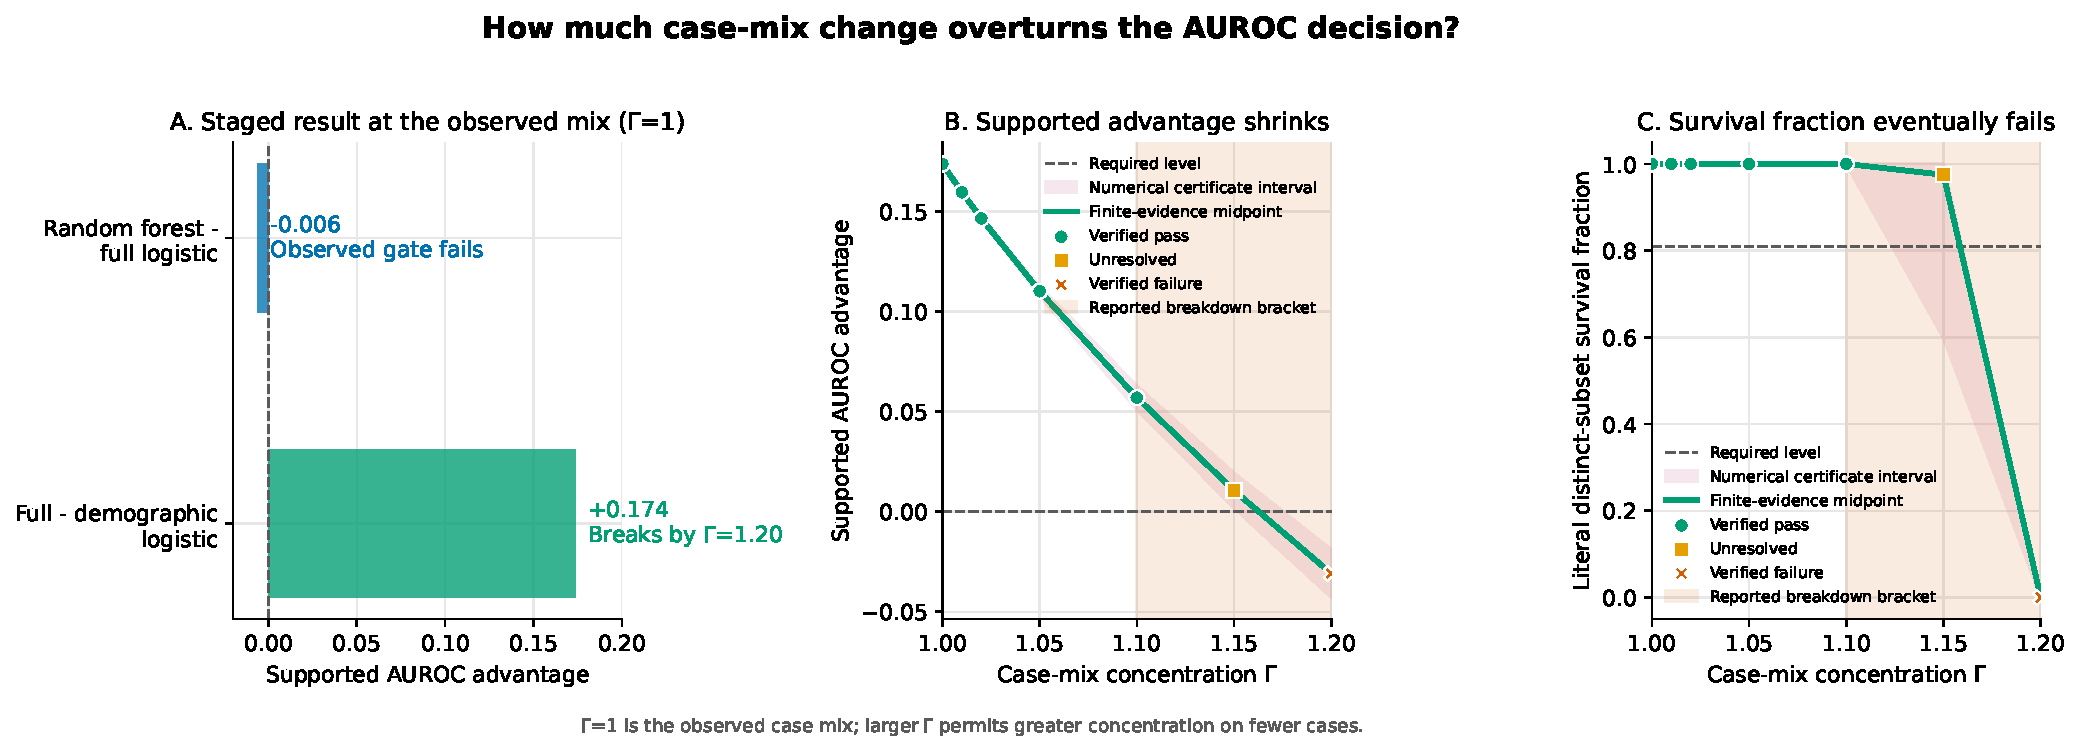
\includegraphics[width=\textwidth]{manuscript_images/banking-auroc-case-mix-breakdown.pdf}
\caption{Observed-anchored AUROC case-mix breakdown in the Bank Marketing
temporal evaluation. Panel A applies the observed gate before the computational
challenge. Panels B and C show the supported-magnitude and literal-survival
profiles for the positive control under increasing within-class concentration.
The ribbon is the numerical certificate interval; markers distinguish verified
passes, unresolved values, and verified failures. The shaded region is the
reported breakdown bracket. This is the $M=1$, $K_E=1$, $K_C=2$, $J=80$
projected boundary of the full construction.}
\label{fig:bank-auroc-case-mix}
\end{figure}

\paragraph{Several empirical evaluations without a computational challenge.}
For ProteinGym, each assay contributed its ordinary paired AUROC difference at
$\Gamma=1$. Applying the declared order-2 empirical challenge gave support
$-0.0663$ for ESM-1v ensemble minus EVE ensemble, $-0.0445$ for ESM-2 650M
minus ESM-1v ensemble, and $-0.0659$ for ESM-2 650M minus EVE ensemble. The
numbers of positive assay effects were respectively $56$, $48$, and $56$ of
$91$, giving exact assay-pair survival fractions $0.376$, $0.275$, and $0.376$.
All three comparisons therefore failed both direct requirements at the
observed mix. The staged rule stopped without within-assay resampling or an
AUROC concentration search. This is the observed-only $M=91$, $K_E=2$,
$K_C=0$ boundary and does not fill the full nested interior.

\begin{figure}[H]
\centering
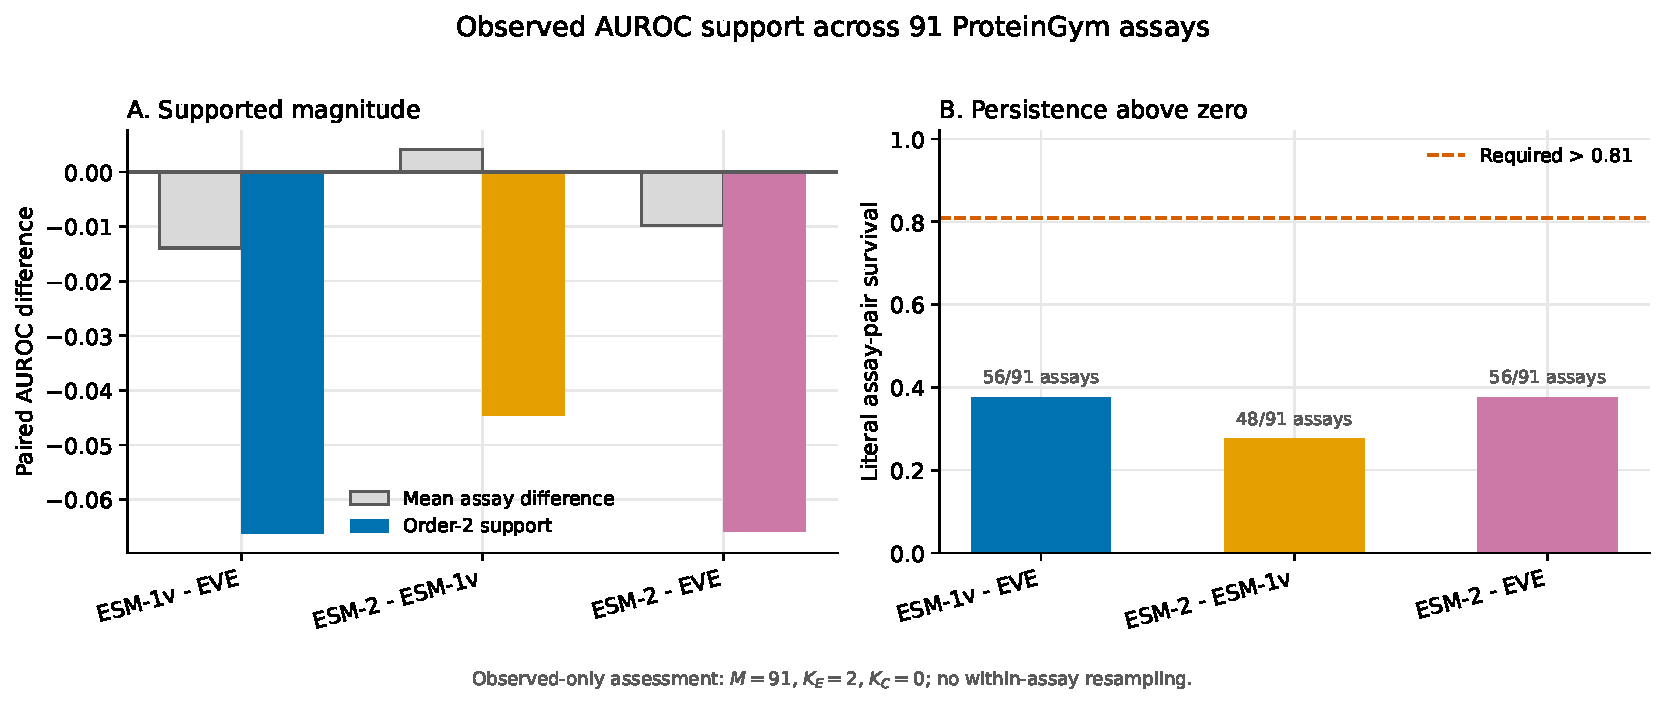
\includegraphics[width=\textwidth]{manuscript_images/proteingym-observed-auroc-decision.pdf}
\caption{Observed-only AUROC support across the 91 ProteinGym assays. Panel A
compares the mean paired assay difference with order-2 supported magnitude.
Panel B gives the exact fraction of the $\binom{91}{2}=4{,}095$ distinct assay
pairs whose two AUROC effects both strictly exceed zero. All comparisons fail
the declared survival requirement. No within-assay computational resampling is
performed.}
\label{fig:proteingym-auroc-decision}
\end{figure}

\subsection{Computation and reporting}

Equation~\eqref{eq:auroc-retained} minimizes the bilinear form
$w_+^\top G w_-$ over two capped simplices. A feasible pair of weights supplies
an upper bound on the infimum and can demonstrate policy failure. Establishing
that the policy continues to hold requires a valid global lower bound;
alternating optimization without such a bound may stop above the true infimum
and overstate survival.

Monotonicity permits a bracketed search over $\Gamma$. Within every searched
value, the global optimization is repeated for each observed anchor and each
required computational cell. The same computational evaluation $D_m^{(j)}$ is
reused throughout the search so that changes in the profile arise from the
concentration allowance rather than from different resamples.

A minimum report gives the Stage 1 result at $\Gamma=1$, the Stage 2 result
when applicable, the breakdown factor, the first failing requirement, the
search tolerance, the global-optimization gap, and Monte Carlo stability for a
computational array. The factor should be labeled full anchored or reduced
observed-only.

Every admissible weight vector redistributes cases already present in an
evaluation. A type absent from that evaluation has weight zero at every
$\Gamma$. Individual reweighting may also concentrate on sample-specific
errors rather than a named subpopulation. The breakdown factor consequently
measures survival under a reproducible empirical concentration rule; it is not
the magnitude of a known deployment shift.


\begin{thebibliography}{99}
\setlength{\itemsep}{0.25em}

\bibitem{acerbi2002spectral}
Acerbi, C. (2002).
Spectral measures of risk: A coherent representation of subjective risk aversion.
\emph{Journal of Banking \& Finance}, 26(7), 1505--1518.

\bibitem{bareinboim2013transportability}
Bareinboim, E., \& Pearl, J. (2013).
A general algorithm for deciding transportability of experimental results.
\emph{Journal of Causal Inference}, 1(1), 107--134.

\bibitem{bestgen2015random}
Bestgen, Y. (2015).
Exact expected average precision of the random baseline for system evaluation.
\emph{The Prague Bulletin of Mathematical Linguistics}, 103, 131--138.

\bibitem{bouckaert2004estimating}
Bouckaert, R. R. (2004).
Estimating replicability of classifier learning experiments.
In \emph{Proceedings of the Twenty-First International Conference on Machine Learning}, 15.

\bibitem{bental2013robust}
Ben-Tal, A., den Hertog, D., De Waegenaere, A., Melenberg, G., \& Rennen, G. (2013).
Robust solutions of optimization problems affected by uncertain probabilities.
\emph{Management Science}, 59(2), 341--357.

\bibitem{chernozhukov2013intersection}
Chernozhukov, V., Lee, S., \& Rosen, A. M. (2013).
Intersection bounds: Estimation and inference.
\emph{Econometrica}, 81(2), 667--737.

\bibitem{cohen1960coefficient}
Cohen, J. (1960).
A coefficient of agreement for nominal scales.
\emph{Educational and Psychological Measurement}, 20, 37--46.

\bibitem{demsar2006statistical}
Dem\v{s}ar, J. (2006).
Statistical comparisons of classifiers over multiple data sets.
\emph{Journal of Machine Learning Research}, 7, 1--30.

\bibitem{duchi2021statistics}
Duchi, J. C., Glynn, P. W., \& Namkoong, H. (2021).
Statistics of robust optimization: A generalized empirical likelihood approach.
\emph{Mathematics of Operations Research}, 46(3), 946--969.

\bibitem{flach2015prg}
Flach, P. A., \& Kull, M. (2015).
Precision-recall-gain curves: PR analysis done right.
In \emph{Advances in Neural Information Processing Systems}, 28.

\bibitem{frazer2021eve}
Frazer, J., Notin, P., Dias, M., Gomez, A., Min, J. K., Brock, K., Gal, Y., \& Marks, D. S. (2021).
Disease variant prediction with deep generative models of evolutionary data.
\emph{Nature}, 599, 91--95.

\bibitem{lipton2018detecting}
Lipton, Z. C., Wang, Y.-X., \& Smola, A. (2018).
Detecting and correcting for label shift with black box predictors.
In \emph{Proceedings of the 35th International Conference on Machine Learning}, PMLR 80, 3122--3130.

\bibitem{lin2023esm2}
Lin, Z., Akin, H., Rao, R., Hie, B., Zhu, Z., Lu, W., et al. (2023).
Evolutionary-scale prediction of atomic-level protein structure with a language model.
\emph{Science}, 379(6637), 1123--1130.

\bibitem{meier2021esm1v}
Meier, J., Rao, R., Verkuil, R., Liu, J., Sercu, T., \& Rives, A. (2021).
Language models enable zero-shot prediction of the effects of mutations on protein function.
In \emph{Advances in Neural Information Processing Systems}, 34, 29287--29303.

\bibitem{moro2014bank}
Moro, S., Rita, P., \& Cortez, P. (2014).
Bank Marketing [Dataset].
UCI Machine Learning Repository. doi:10.24432/C5K306.

\bibitem{nadeau2003inference}
Nadeau, C., \& Bengio, Y. (2003).
Inference for the generalization error.
\emph{Machine Learning}, 52, 239--281.

\bibitem{notin2023proteingym}
Notin, P., Kollasch, A., Ritter, D., van Niekerk, L., Paul, S., Spinner, H., et al. (2023).
ProteinGym: Large-scale benchmarks for protein fitness prediction and design.
In \emph{Advances in Neural Information Processing Systems}, 36, Datasets and Benchmarks Track.

\bibitem{popper1959logic}
Popper, K. R. (1959).
\emph{The Logic of Scientific Discovery}.
Hutchinson.

\bibitem{popper1963conjectures}
Popper, K. R. (1963).
\emph{Conjectures and Refutations: The Growth of Scientific Knowledge}.
Routledge.

\bibitem{saerens2002adjusting}
Saerens, M., Latinne, M., \& Decaestecker, C. (2002).
Adjusting the outputs of a classifier to new a priori probabilities.
\emph{Neural Computation}, 14(1), 21--41.

\bibitem{siblini2020calibration}
Siblini, W., Fr\'ery, J., He-Guelton, L., Obl\'e, F., \& Wang, Y. (2020).
Master your metrics with calibration.
In \emph{Advances in Intelligent Data Analysis XVIII}, 457--469.

\bibitem{shapiro2017distributionally}
Shapiro, A. (2017).
Distributionally robust stochastic programming.
\emph{SIAM Journal on Optimization}, 27(4), 2258--2275.

\bibitem{storkey2009training}
Storkey, A. (2009).
When training and test sets are different: characterizing learning transfer.
In \emph{Dataset Shift in Machine Learning}, 3--28. MIT Press.

\bibitem{wang1996premium}
Wang, S. (1996).
Premium calculation by transforming the layer premium density.
\emph{ASTIN Bulletin}, 26(1), 71--92.

\end{thebibliography}

\end{document}
